\chapter{Statistical Shape \& Appearance Modelling}\label{PCA_CHAP}

\section{Introduction}

Statistical shape and appearance models give the opportunity to investigate the
consequences of variation in a dataset that otherwise would be difficult to
isolate or obtain enough experimental specimens to find trends in the data.
The effect of the anterior height of the vertebral body on the response to
loading is a simple example of this. In this example, to understand the effect
of anterior vertebral height experimentally, or computationally using specimen
specific models, a large range of vertebrae with varying anterior heights would
be required which would hopefully represent (without gaps) the range of
anterior heights in the population. Even if this could be achieved, confounding
factors and other variation would make the presentation of specific
relationships difficult. Using statistical shape and appearance models with
principal component analysis (PCA), the modes of variation can be characterised
and isolated, allowing an understanding of how specific modes of variation
affect the chosen measure. A caveat here (similar to specimen specific models,
but potentially less obvious) is that the modes of variation are specific to
the input set, the models used to make the statistical shape models. Hence, any
estimations of the types of variation and the effects these modes of variations
have is specific to that set of models and not necessarily applicable to the
population on the whole.

This chapter focusses on using the 14 human lumbar vertebra FE model from the previous
chapter as the input set to create a statistical shape and appearance model
based upon them. Specifically, this chapter describes the methods used to
create the statistical models and aims to find the main modes of variation found within the
input set. These modes of variation are then validated, ensuring the variation
found in generated models based on the statistical shape model are within the
realms of possibility, given the input set they are created from. Finally the
generated models are artificially augmented, using the results of the previous
chapter, in order to start to understand how material and geometric properties
of vertebrae effect the outcomes of vertebroplasty.

\subsection{Aims of Statistical Shape \& Appearance Models}

\subsection{General Methodology}

Generally SSAMs start with a rigid registration, where rotations and
translations are applied to all meshes or models that form the input data set
so that they share a common coordinate system.  Methods of performing the rigid
registration often use an automated approach where certain degrees of freedom
are restricted to ensure registration is achieved.



\section{Methods}

\subsection{Measuring Vertebral Geometry}

Vertebral volume or the vertebral body volume may be the easiest and most
obvious measure of geometric change within a set of vertebra.  It has been
shown in \cref{Chapter_HT} that there is a strong correlation between
vertebral size and stiffness and so this may be enough for a range of
comparisons between spines and individual vertebrae.  However, the input set of
vertebrae contain a wide range of variation which can be seen visually, which
may play an important role in the effect of cement augmentation and is another
method of validating the outputs from the PCA generated set of models.

Measuring vertebral geometries in previous studies have either taken the
measurements from x-ray scans \cite{Gilad1986,Gilad1985} or $\mu$CT scans
\cite{Zhou2000,Cheung1994}, where the measurements have been made through the
moving a cursor to the locations of specific points and reporting the distance
between them.  While this method may produce accurate results, there is
inherent human error associated, the number of measurements is limited to the
number of planes available and applying this to large sets of data is time
consuming which may lead to further error.

The approach used here involves using the 1 mm voxel resolution models
generated in ScanIP (v. 2016) which are are used for FE modelling.  The mask
describing the vertebral body of these vertebrae is exported as a
stereolithography file (STL), allowing the surface of the vertebra to be
measured.  Measuring the vertebra was carried out in Matlab where the STL file
was imported forming a point cloud describing the surface from the surface
nodes.  Once imported the point cloud was split into thirds in each of the
three anatomical planes, with the points describing the vertebra within these
thirds being stored in nine array variables.  Cuboids were then fitted to the
3D arrays, maintaining the correct alignment and therefore prohibiting rotation
of the cuboid.  The cuboid fits can be seen in \cref{fig:cuboid_ax,
fig:cuboid_sag, fig:cuboid_cor}.


\begin{figure}[ht!]
  \centering
  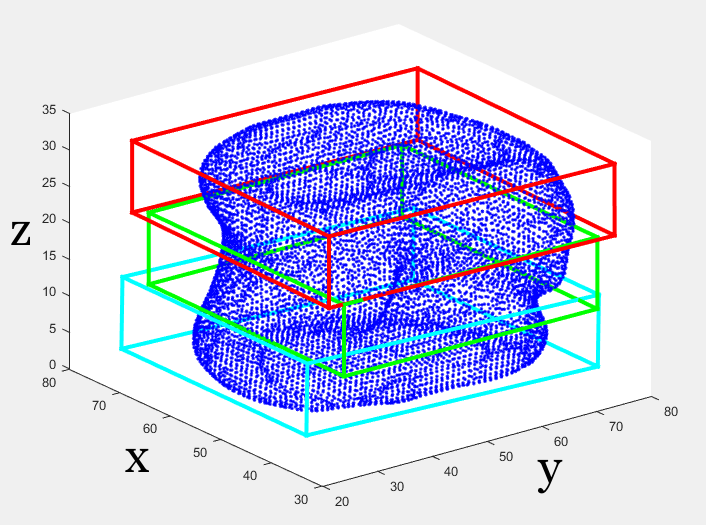
\includegraphics[width=4in]{Chapters/Chapter_PCA_images/Cuboid_fit_axial.png}
  \caption{The three cuboids fitted to the vertebra point cloud in the axial plane.}
  \label{fig:cuboid_ax}
\end{figure}

\begin{figure}[ht!]
  \centering
  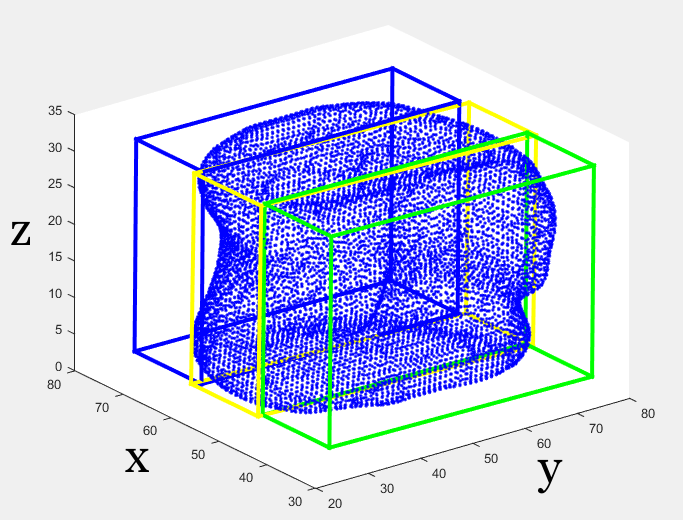
\includegraphics[width=4in]{Chapters/Chapter_PCA_images/Cuboid_fit_coronal.png}
  \caption{The three cuboids fitted to the vertebra point cloud in the coronal plane.}
  \label{fig:cuboid_cor}
\end{figure}

\begin{figure}[ht!]
  \centering
  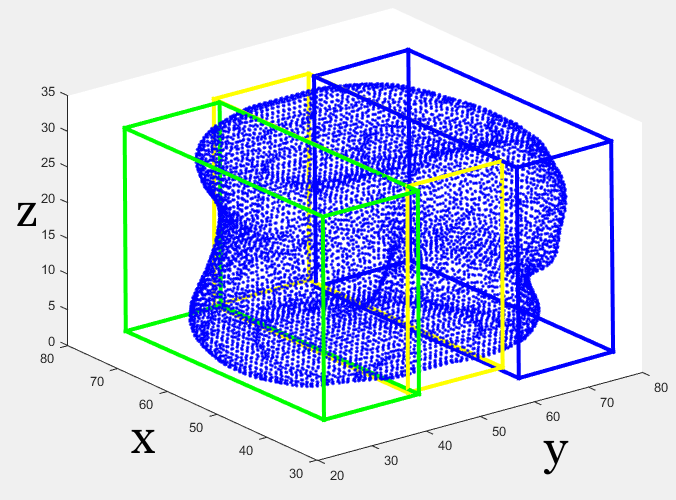
\includegraphics[width=4in]{Chapters/Chapter_PCA_images/Cuboid_fit_sagital.png}
  \caption{The three cuboids fitted to the vertebra point cloud in the sagital plane.}
  \label{fig:cuboid_sag}
\end{figure}

Measuring the two longer sides of the fitted cuboids gives a total of 18
measurements describing most aspects of the vertebral geometry, these can be
seen with their abbreviations in Table \ref{tab:measurements}.  This includes
identifying wedge shaped vertebrae, recorded as reduced anterior height
compared to the posterior height, left to right wedge shapes, recorded as
sagital left height being smaller or larger when compared to the sagital right
height.

\begin{table}[ht!]
	\caption{The measurements and abbreviations taken from the vertebrae.}
	\label{tab:measurements}
	\centering
	\begin{tabular}{c|c}
    Measurement & Abbreviation \\
    \hline
    \hline
    Sagital Left Height & SLH \\
	Sagital Left Depth & SLD \\
    Sagital Mid Height & SMH \\
	Sagital Mid Depth & SMD \\
    Sagital Right Height & SRH \\
	Sagital Right Depth & SRD \\
	Coronal Anterior Height & CAH \\
	Coronal Anterior Width & CAW \\
	Coronal Mid Height & CMH \\
	Coronal Mid Width & CMW \\
	Coronal Posterior Height & CPH \\
	Coronal Posterior Width & CPW \\
	Axial Inferior Depth & AID \\
	Axial Inferior Width & AIW \\
	Axial Mid Depth & AMD \\
	Axial Mid Width & AMW \\
	Axial Superior Depth & ASD \\
	Axial Superior Width & ASW \\
	\hline
	\end{tabular}
\end{table}

The plugin for ScanIP that allows principal component analysis and the
generation of models described by the principal components consists of five
main steps.

The first of these steps is a pre-processing step, converting the masks and
backgrounds into nessessary formats (.mha \& .mhd) for use with the ITK
toolkit.

The following step carries out rigid registration of the models, aligning the
masks and backgrounds to a shared coordinate system.  This is carried out using
the ITK library with the registration being measured according to a mean
squared image-to-image metric using a gradient descent optimiser.  A limit to
the number of attempts or steps allowed can be set; the default value of 100
steps for each input model was used.

The geometry of each input specimen was described in a deformable registration
step, measuring the transform required to morph the mean of the input vertebrae
onto each of the input vertebrae.  This step utilises the ITK FEM registration
filter.

Penultimately, the transforms between the mean and each of the input vertebrae
which describe the vertebral geometries are used as inputs for PCA.  Here the
outputs of the step include the principal components, their eigenvalue,
percentage of variation captured in that component and the cumulative
percentage variation captured.

Finally, the SSAM produced can be used with the ITK Image Warp filter to
generate new mask and background combinations from within the envelope of
geometric and material property variation created by the input set, according
to the principal components.  The plugin allows for the first five principal
components (PC1, PC2, PC3, PC4 \& PC5) to be used for as variables for model
generation, altering the value of the principal components by up to three
standard deviations away from the mean in both positive and negative
directions.

\subsection{Generating Vertebrae Models}

\subsubsection{Range of Shapes Generated}

To attempt to understand what each of the principal components represented in
terms of the variation captured by it, models were created at $\pm$1, $\pm$2
and $\pm$3 standard deviations away from the mean for the first three principal
components independently.  In addition to these, the mean model was generated,
allowing comparisons of the other generated models against it.

Finally, in order to know whether the range of geometries, material properties
and resultant stiffnesses found in the input set was represented in the SSAM
within the first three principal components, models were generated which
incorporated the variation found in PC1, PC2 \& PC3.  These models would
represent the corners of a cube who's axis would be PC1, 2 \& 3 and who's
origin would be the mean vertebra.  If the majority of input models (68 \%,
representing the quantity of the population expected to fit within $\pm$1 SD of
the mean for a normally distributed input set) fit within the limits created by
a cube with side length from +1 to -1 SD along each axis for geometric
measurements, greyscale background and resultant stiffness, then the variation
of the input set will have been captured and represented by the SSAM.

\subsubsection{FE Model Setup}

Once the vertebrae were generated using the plugin the rest of the FE model was
set up.  This included forming endcaps to mimic the experimental setup and how
the input set was loaded.  Endcaps were created programmaticaly within the
ScanIP python scripting environment with a diameter of 90 mm, approximately
equal to the diameter of the experimental endcaps, with a depth of 6 mm
ensuring the superior and inferior tips of the vertebrae were captured with a
minimum of 1 mm between the vertebra and end of the cement.  The remaining
properties for the FE model are identical to those used for the models of the
human vertebra which became the inputs to the PCA plugin.  This includes a tied
interaction between the vertebrae and endcaps and material properties for the
endcaps being: Young's modulus 2.45 GPa and Poissons's ratio of 0.3.  Material
properties for the vertebra used the same greyscale approach as in previous
chapters with the Young's modulus for each element being: \[ E = GS \times
\alpha \] Where, $GS$ is the greyscale value for the current element (between 0
and 255) and $\alpha$ is the conversion factor.  The conversion factor used has
the same value used previously for the non-augmented set of vertebrae: $\alpha
= 0.0008184$.  Applying load to the models is carried out as in the previous
chapter, with 1 mm of displacement applied to a loading point, with the
reaction force being measured to obtain the stiffness.  The loading point is
found by finding the centre of the vertebral body in the middle slice axially
and translating the point axially to the maximum height of the model, including
endcaps.  The load is then applied through a plate which is tied to the
superior endcap.

\subsubsection{Augmentation in Generated Models}




\section{Results}

\subsection{Validating Generated Vertebrae} \label{sec:pca_val}

Validation of the generated vertebrae from the PCA plugin for scanIP is vital
for ensuring any results are sensible, for example when artificially augmenting
the vertebrae, and to ensure that the modes of variation previously described
are genuine descriptions of the variation found within the input set.  To
achieve this validation, aspects important to the generated models need to be
compared to the variables found in the input set.  The variables compared will
be the geometry and volume of the vertebrae, the greyscale background and
therefore the material properties of the models and finally the resulting
stiffness when loads are simulated on the generated FE model.  While
identifying the modes of variation in isolation are important to characterise
how such variation affects the outcomes of augmentation or understanding the
content and main modes of variation, combinations of the principal components
generate different models that may describe different ranges of variation.
Therefore, the variation found within one standard deviation of the mean for
the first three principal components, including all of the combinations of
standard deviations within $\pm$ 1 SD, including the mean.  For example, PC 1
+1, PC 2 +1, PC 3 -1, would be one model with a combination of the first three
principal components.

\subsubsection{Geometry Validation}

Identifying the variation in geometry for combinations of the first three
principal components, with all possible combinations within $\pm$1 SD of the
mean is presented here.  The 18 geometric measures found within the $\pm$1 SD
models are presented in \cref{fig:pca_cube}.  The results presented here show a
strong agreement between the input and the generated models, with the means of
the two sets agreeing closely, along with the range of the measurements.
Outliers in the input set originate from the bone spurs and other features of
the degenerated vertebrae. %TODO add image of G19 L1 Differences in the range
of generated vertebrae compared to the range of measurements seen in the input
set are due to the input set describing only one standard deviation of
variation.

Volume differences between the input set and generated vertebrae were also
small, with the difference between the mean of the input set volume and the
mean generated model volume being 10 \%, the means being 39500 mm$^3$ and 38245
mm$^3$ respectively.  The range of vertebral volumes is also comparable: the
input set range is 31189 to 56003 mm$^3$ while the generated vertebrae for
$\pm$1 SD with all possible combinations of PC 1, 2 and 3, have a range of
28152 to 50462 mm$^3$.

\begin{figure}[h!]
  \centering
  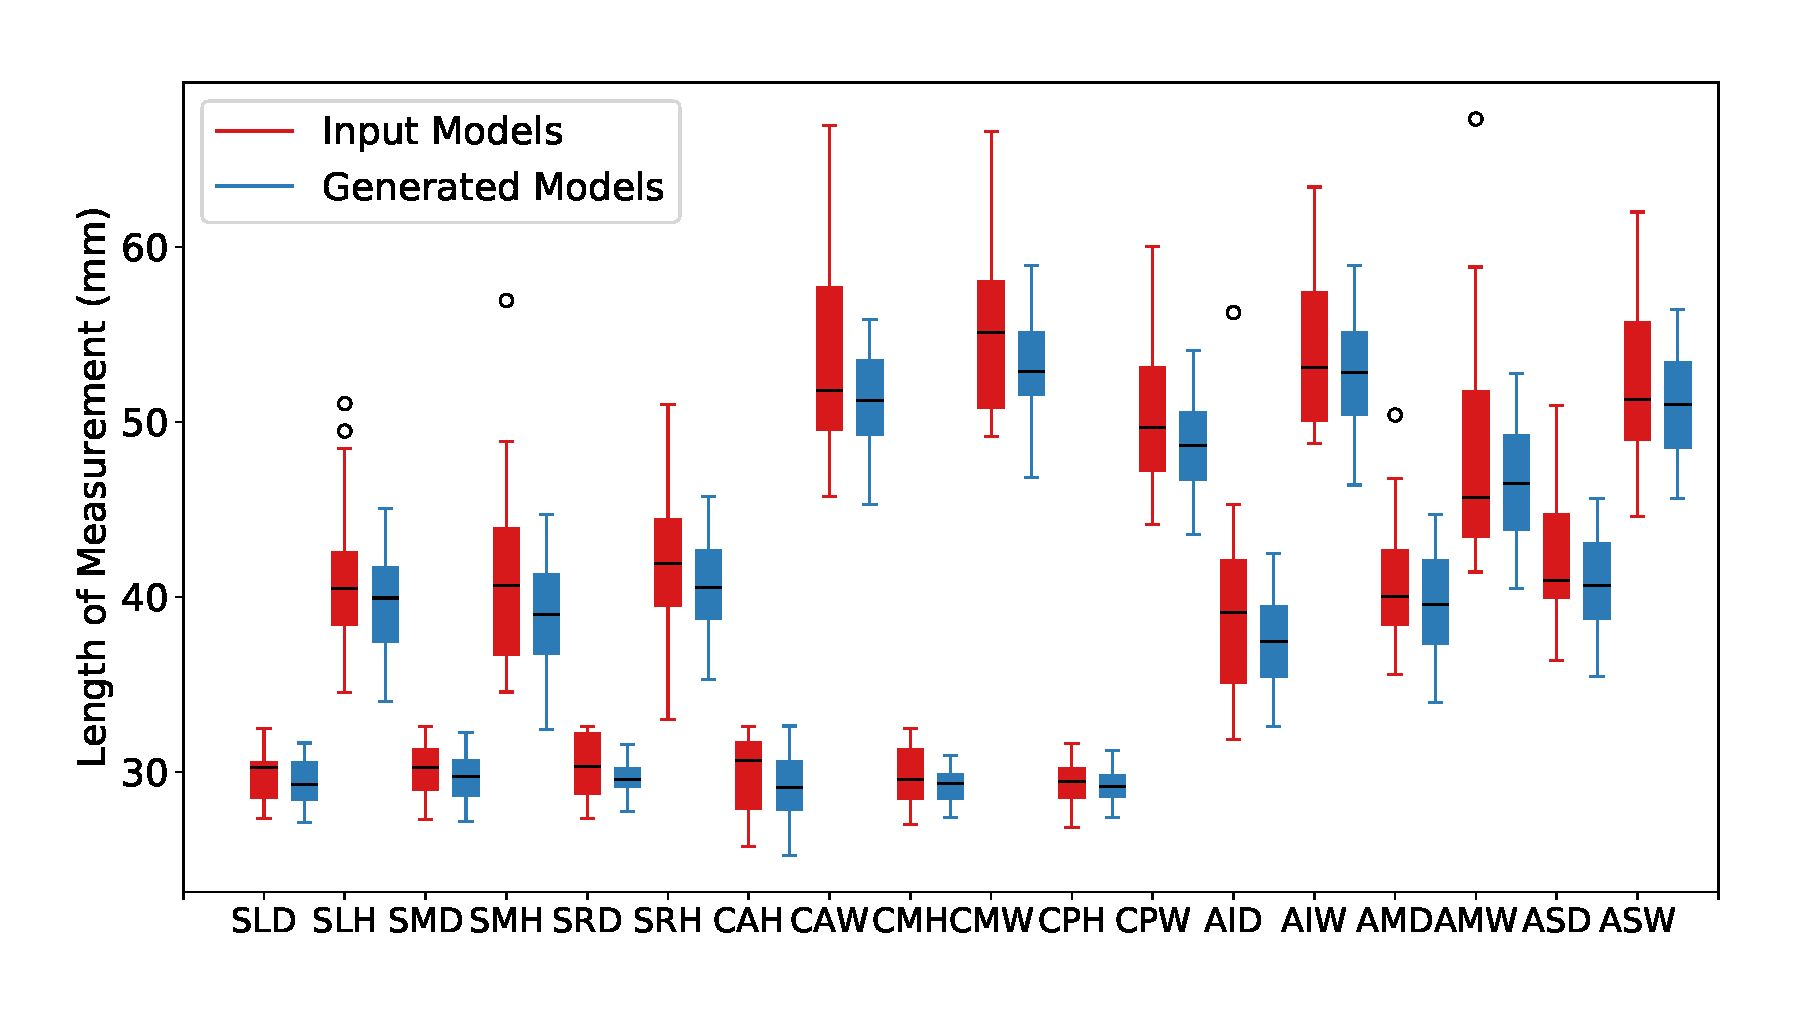
\includegraphics[width=\textwidth]{Chapters/Chapter_PCA_images/pca_cube.pdf}
	\caption[Geometric variation in the generated vertebrae.]{The variation in the 18 geometric measures of the input set models compared to the variation in the generated models for the first three principal components including all combinations of the +1, mean and -1 standard deviations.}
  \label{fig:pca_cube}
\end{figure}

\subsubsection{Material Property (Greyscale) Validation}


The variation seen in the histograms representing the greyscale differences
between generated models and the input can be seen in
\cref{fig:pca1_histo,fig:pca2_histo,fig:pca3_histo}, with the range of
histograms from the input set shown as the grey range and the coloured lines
showing the histogram for each of the generated models.  This normalised data
shows a general agreement with the shape of the curves and relative quantities
being very similar.  Deviations from the similarity are, for the most part, at
the high and low greyscale values, where in general there are less voxels in
this range for the generated models.  Comparing these results to an example
background in \cref{fig:input_gen_background}, comparing an input background
slice with the mean generated model mid-slice, shows that the lack of voxel
counts in the high and low greyscale regions correlates with having less
contrast between the densest bone in the cortical shell and the empty parts.
Additionally, \cref{fig:input_gen_background} shows that the important feature
for load transfer, the cortical shell, is preserved and accurately described in
the background of the mean generated model.  While the cortical shell's
presence is clear, it's definition and contrast between it and the trabecular
bone or empty spaces is not as well preserved.  Other features such as the
posterior vascular channel is also preserved, albeit not as clearly as the
features on the input set.

Differences in the mean greyscale between the input set and the generated
models of all combinations of $\pm$1 SD are 108 and 97 respectively.  The
ranges are 78 to 164 for the input set and 72 to 122 for the generated models
for all combinations of $\pm$1 SD.
\begin{figure}[h!]
  \centering
  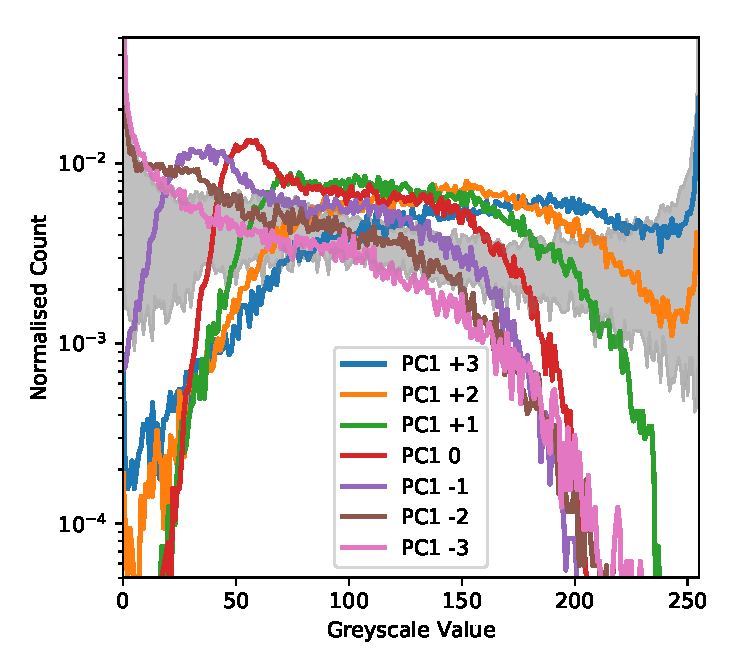
\includegraphics[width=.65\textwidth]{Chapters/Chapter_PCA_images/pca1_histo.pdf}
  \caption{Histogram of the models generated from principal component 1, with $\pm$ 3, 2 \& 1 standard deviations away from the mean. The values are normalised with respect to the total volume of the vertebrae, allowing comparisons with different sized model. The grey background represents the range of histograms seen in the input set.}
  \label{fig:pca1_histo}
\end{figure}

\begin{figure}[h!]
  \centering
  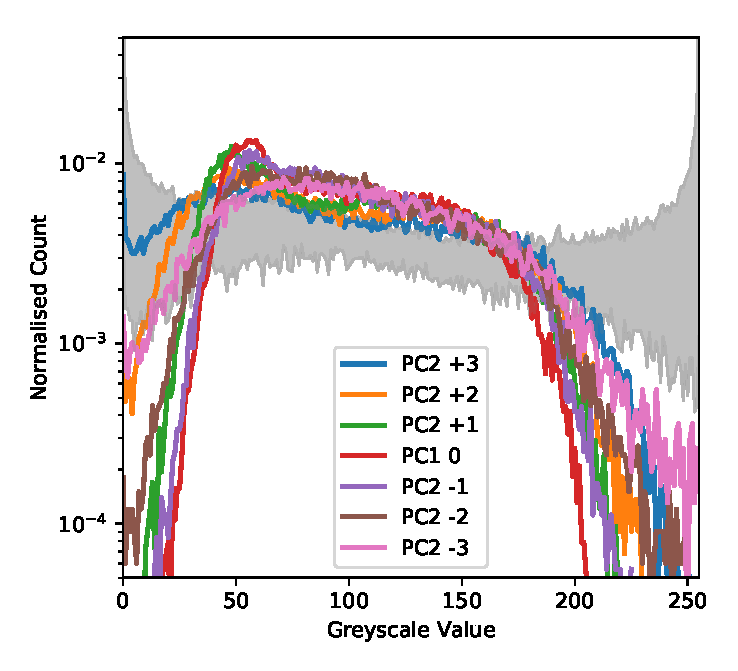
\includegraphics[width=.65\textwidth]{Chapters/Chapter_PCA_images/pca2_histo.pdf}
  \caption{Histogram of the models generated from principal component 2, with $\pm$ 3, 2 \& 1 standard deviations away from the mean. The values are normalised with respect to the total volume of the vertebrae, allowing comparisons with different sized model. The grey background represents the range of histograms seen in the input set.}
  \label{fig:pca2_histo}
\end{figure}

\begin{figure}[h!]
  \centering
  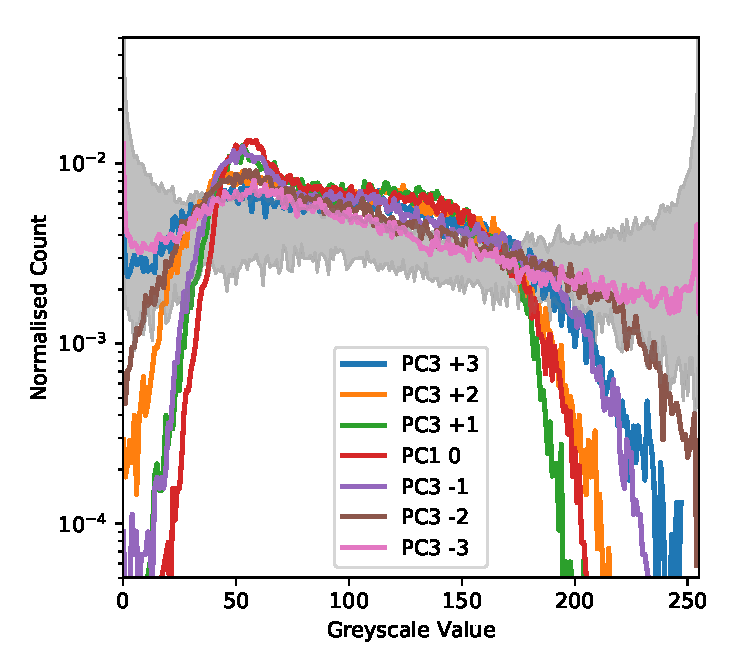
\includegraphics[width=.65\textwidth]{Chapters/Chapter_PCA_images/pca3_histo.pdf}
  \caption{Histogram of the models generated from principal component 3, with $\pm$ 3, 2 \& 1 standard deviations away from the mean. The values are normalised with respect to the total volume of the vertebrae, allowing comparisons with different sized model. The grey background represents the range of histograms seen in the input set.}
  \label{fig:pca3_histo}
\end{figure}

\begin{figure}[h!]
  \centering
  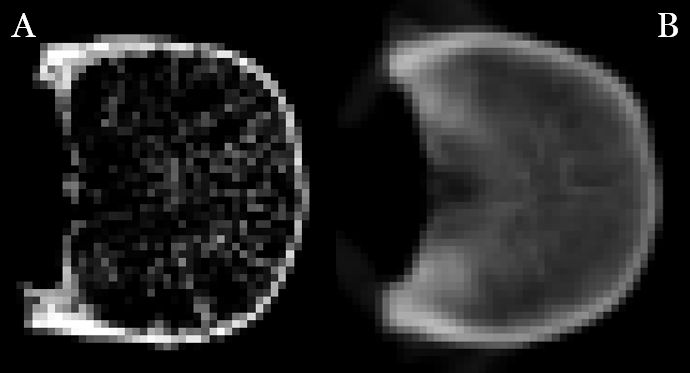
\includegraphics[width=.6\textwidth]{Chapters/Chapter_PCA_images/INPUT_GEN_BACKGROUND.png}
	\caption{Greyscale backgrounds for the axial mid-slice from, A, the Spine 1 L1 input vertebra and B, the mean generated model.}
  \label{fig:input_gen_background}
\end{figure}
\subsubsection{Resulting Stiffness Validation}

The range of stiffness values from the generated models from all possible combinations of the first three principal components within 1 standard deviation matched closely with the range of stiffness' from the input set. These were 2791 - 6039 N/mm and 2887 - 6172 N/mm for the input and generated models respectively. Additionally the means of the sets also agreed well with the mean computational stiffness of the input set being 4508 N/mm and 4134 N/mm for the mean generated model.

\begin{table}[h]
\centering
\caption{The stiffness of the generated models from PC1, 2 and 3, showing the fractional change to the mean model in each case.}
\label{tab:stiffness_gen_models}
\begin{tabular}{c|c|c}
Model  & Stiffness (N/mm) & Fractional Change from the Mean \\ \hline \hline
PC1 +3 & 6543.38          & 1.582                           \\
PC1 +2 & 5887.75          & 1.424                           \\
PC1 +1 & 5059.89          & 1.224                           \\
Mean   & 4134.88          & 1.000                           \\
PC1 -1 & 2962.82          & 0.717                           \\
PC1 -2 & 1696.47          & 0.410                           \\
PC1 -3 & 1131.86          & 0.274                           \\ \hline
PC2 +3 & 4159.29          & 0.980                           \\
PC2 +2 & 4291.53          & 0.831                           \\
PC2 +1 & 4355.98          & 0.770                           \\
Mean   & 4134.88          & 1.000                           \\
PC2 -1 & 4051.57          & 1.006                           \\
PC2 -2 & 3434.91          & 1.038                           \\
PC2 -3 & 3182.81          & 1.053                           \\ \hline
PC3 +3 & 2930.69          & 0.709                           \\
PC3 +2 & 3420.55          & 0.827                           \\
PC3 +1 & 3846.57          & 0.930                           \\
Mean   & 4134.88          & 1.000                           \\
PC3 -1 & 4409.05          & 1.066                           \\
PC3 -2 & 4240.58          & 1.026                           \\ \hline
PC3 -3 & 4141.31          & 1.002                          
\end{tabular}
\end{table}


\subsection{Measuring \& Interrogating Vertebral Variation}

\subsubsection{Geometry Variation}

The geometric variation found in the first three principal components has been
identified using the images of the surface point clouds of the mean and +3 and
-3 standard deviations away from the mean, along with the measurements of the
18 variables described previously.  The images of the point clouds can be seen
in \cref{fig:PC1_2_3_Axial,fig:PC1_2_3_Sagital,fig:PC1_2_3_Coronal}, showing
the view of the vertebral models from the three anatomical planes with a
three-dimensional view in \cref{fig:PC1_2_3_3D}.  More simplified figures can
be seen in
\cref{fig:PC1_2_3_AxialSlice,fig:PC1_2_3_SagitalSlice,fig:PC1_2_3_CoronalSlice},
showing the mid-slice through each of the anatomical planes, while information
is lost here, it allows an clear visualisation of the modes of variation found
in the main parts of the vertebral body.  Here, only the +3, mean and -3
standard deviations of the principal components are shown, this simplifies and
allows clear visualisations of the main mode of variation present in each
principal component.  A quantification of the change in volume can be seen in
\cref{tab:pca_geo_tab} for the mean and $\pm$ 1, 2 \& 3 standard deviations
away from the mean.

Principal component one contains the least geometric variation of the first
three principal components.  The mid slice axially shows an almost identical
shape and size between the +3, mean and -3 standard deviations, while the
coronal and sagittal planes show minor changes in the overall size and volume
of the vertebrae.  The changes in total vertebral volume is limited to 17 \%
larger and 15 \% smaller than the mean model, shown in \cref{tab:pca_geo_tab}.

Principal component two shows the most interesting geometric variation with
many of the different shapes and some of the degeneration of the input set
clearly visible.  The large changes to the axial mid slice
(\cref{fig:PC1_2_3_AxialSlice}) of the second principal component appear to
represent the different levels of the lumbar spine that made up the input set.
Positive standard deviations away from the mean, especially the +3 SD slice has
the much wider posterior portion aligning with that of the L5 lumbar vertebrae.
Conversely the much narrower -3 SD model appears similar to the L1 lumbar
vertebrae.  This change in width between the +3 and -3 SD is especially evident
in the coronal views in \cref{fig:PC1_2_3_CoronalSlice}.  This change from
vertebra reminiscent of L5 vertebrae at +3 SD to L1 vertebra at -3 SD (and
therefore L3 vertebrae in the mean model) is also reflected in the sagittal
views (\cref{fig:PC1_2_3_SagitalSlice}) where anterior and posterior wedge
shapes can be seen in the +3 and -3 SD models respectively.

Finally, principal component three also contains a considerable quantity of the
geometric variation, although much more simple.  Here, the mode of geometric
variation is the size of the vertebrae with the -3 SD model being considerably
larger than the mean vertebral model (54 \% larger) and vice versa with the +3
SD model, where its volume is much smaller than the mean vertebra (40 \%
smaller).

Quantification of all of the measurements taken on the generated models can be
seen in \cref{tab:pca_geo_tab} with the acronyms for the measurements given in
\cref{tab:measurements}.  The colouration in the table allows easy
identification of the changes to the vertebral geometry compared to the mean
generated model, for example, while the changes to the measurements are near
uniform in PC 1 \& 3, the non-uniform nature of PC 2 shows the different shapes
that are present and described above.  Additionally it allows quantification of
the shapes seen in the models, for example the anterior and posterior wedge
shapes in PC 2, described with the Coronal Anterior Height and the Coronal
Posterior Height having an antagonistic relationship.  However, the main
benefit of the table and its measurements is for the validation of the PC
models against the input set, ensuring that the shapes measured in the input
set are represented in the models.  This is described in \cref{sec:pca_val}.


%\begin{figure}[p]
%  \centering
%  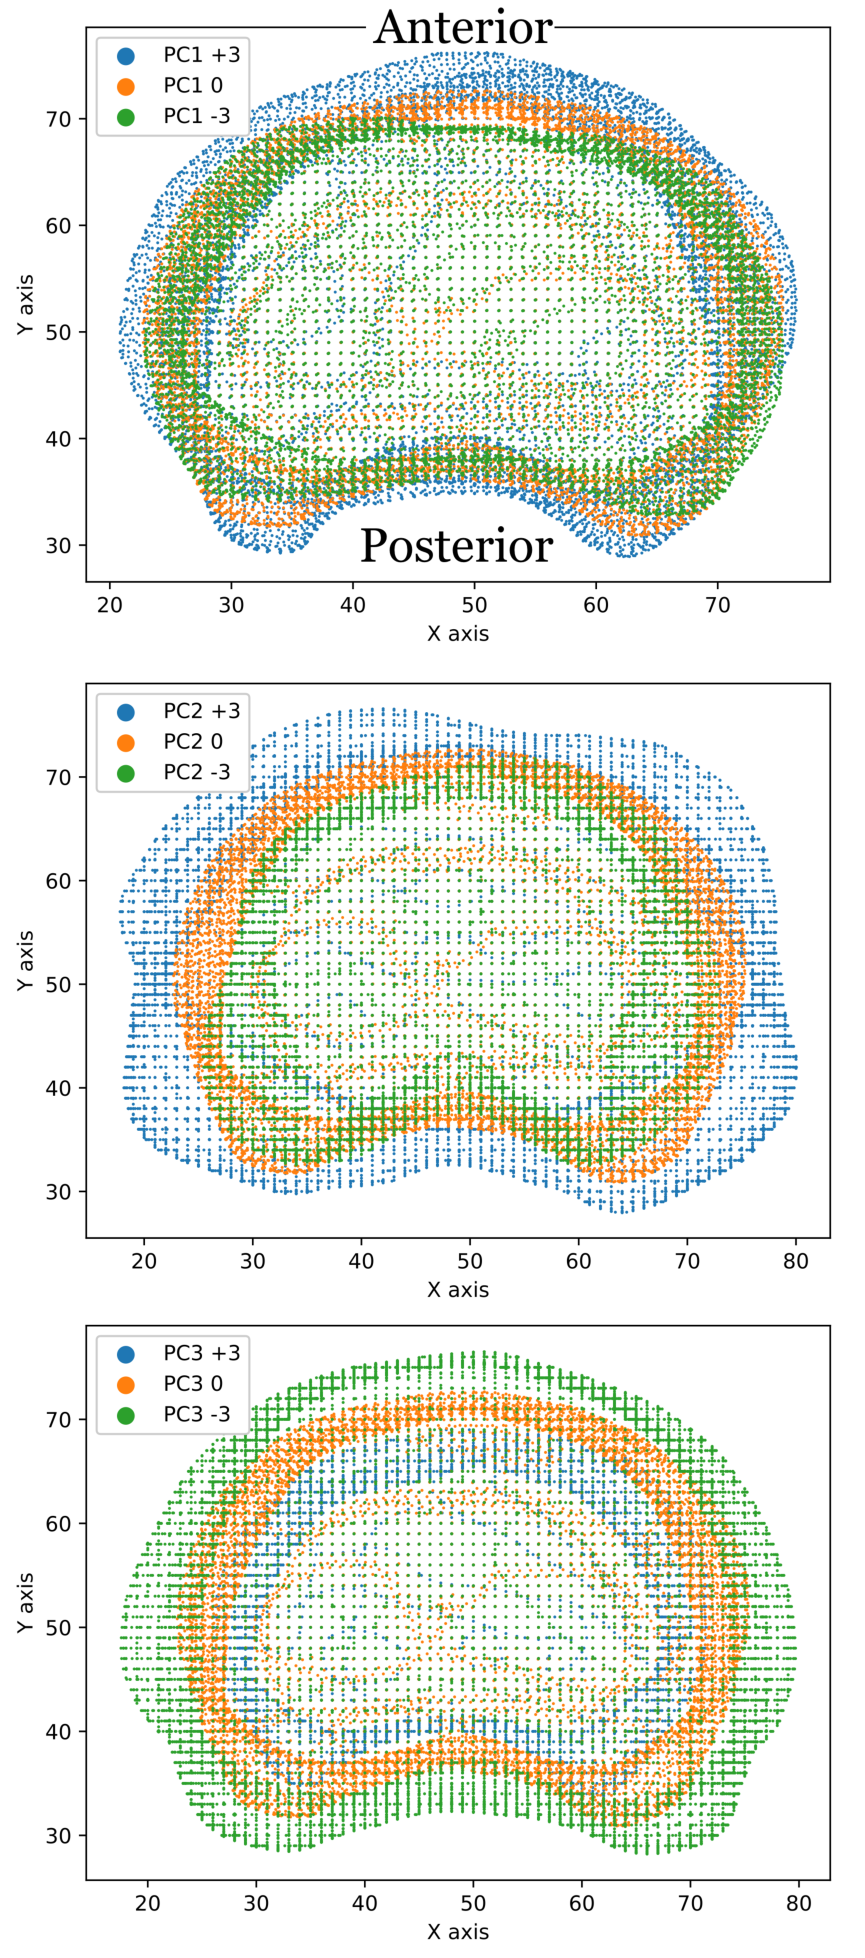
\includegraphics[width=.65\textwidth]{Chapters/Chapter_PCA_images/PC1_2_3_Axial.pdf}
%  \caption{Axial views of the surface point clouds of the vertebral models from the first three principal components, showing the mean, +3 and -3 standard deviations away from the mean. Showing how the geometry is captured in the first three principal components.}
%  \label{fig:PC1_2_3_Axial}
%\end{figure}
%
%\begin{figure}[p]
%  \centering
%  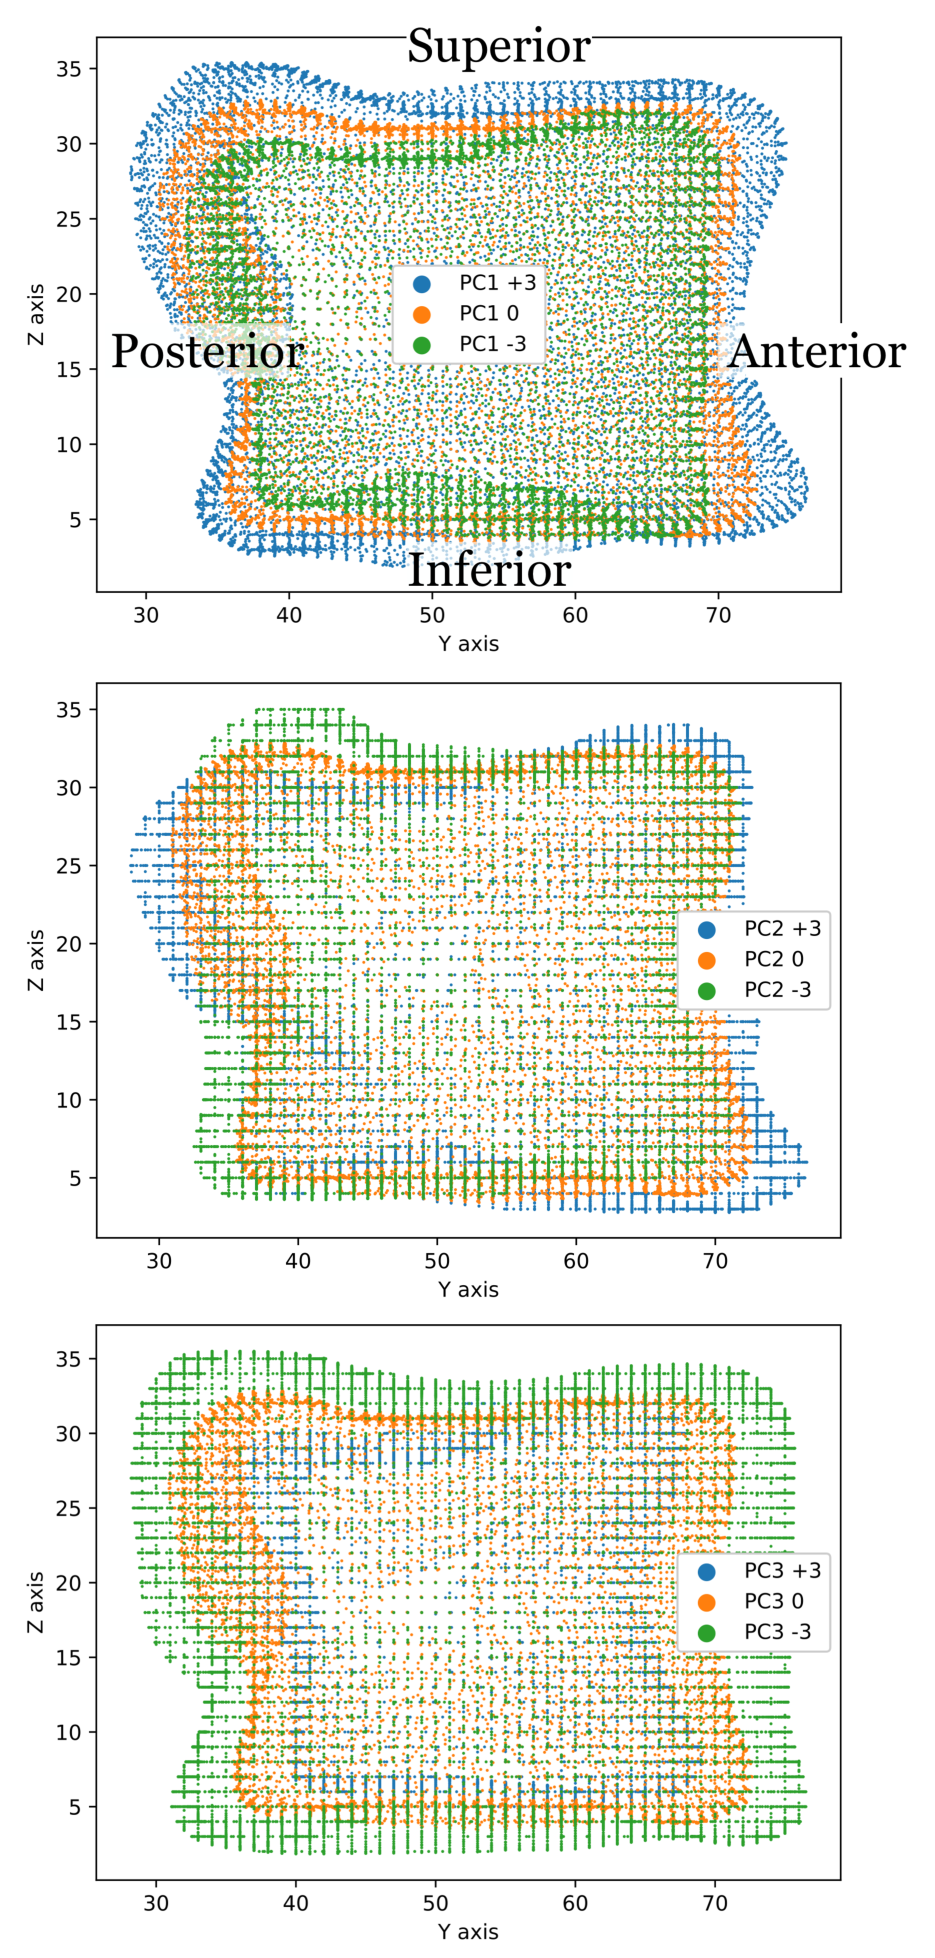
\includegraphics[width=.65\textwidth]{Chapters/Chapter_PCA_images/PC1_2_3_Sagital.pdf}
%  \caption{Sagittal views of the surface point clouds of the vertebral models from the first three principal components, showing the mean, +3 and -3 standard deviations away from the mean. Showing how the geometry is captured in the first three principal components.}
%  \label{fig:PC1_2_3_Sagital}
%\end{figure}
%
%\begin{figure}[p]
%  \centering
%  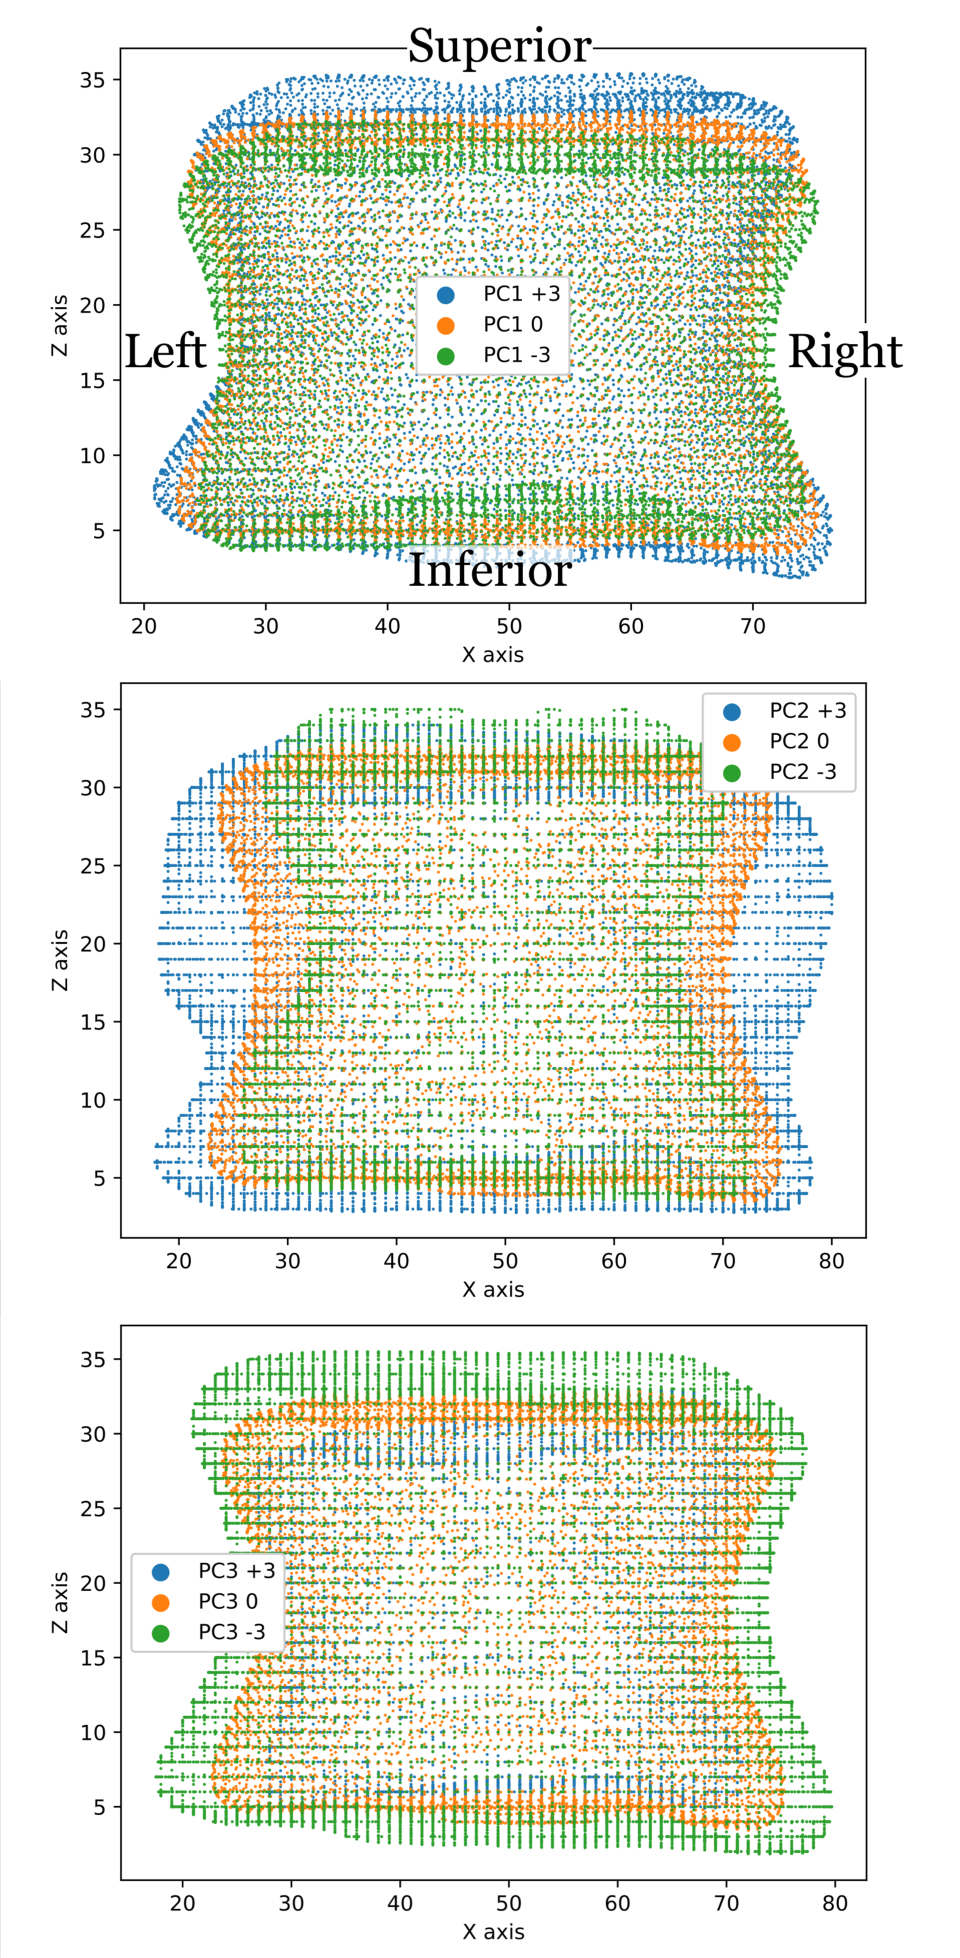
\includegraphics[width=.65\textwidth]{Chapters/Chapter_PCA_images/PC1_2_3_Coronal.pdf}
%  \caption{Coronal views of the surface point clouds of the vertebral models from the first three principal components, showing the mean, +3 and -3 standard deviations away from the mean. Showing how the geometry is captured in the first three principal components.}
%  \label{fig:PC1_2_3_Coronal}
%\end{figure}



\begin{figure}[p]
  \centering
  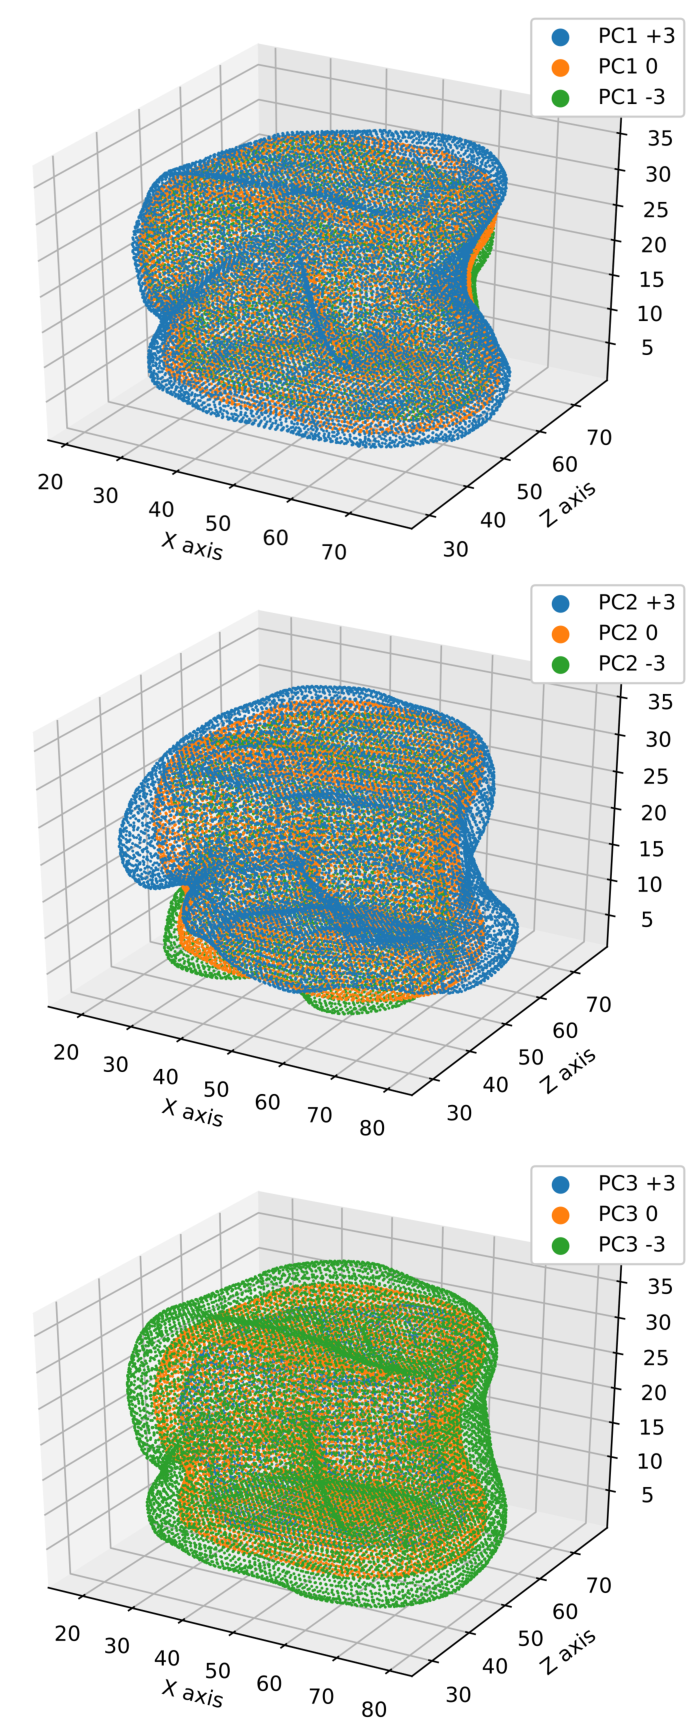
\includegraphics[width=.65\textwidth]{Chapters/Chapter_PCA_images/PC1_2_3_3D.pdf}
  \caption{Three dimensional views of the surface point clouds of the vertebral models from the first three principal components, showing the mean, +3 and -3 standard deviations away from the mean. Showing how the geometry is captured in the first three principal components.}
  \label{fig:PC1_2_3_3D}
\end{figure}


\begin{figure}[p]
  \centering
  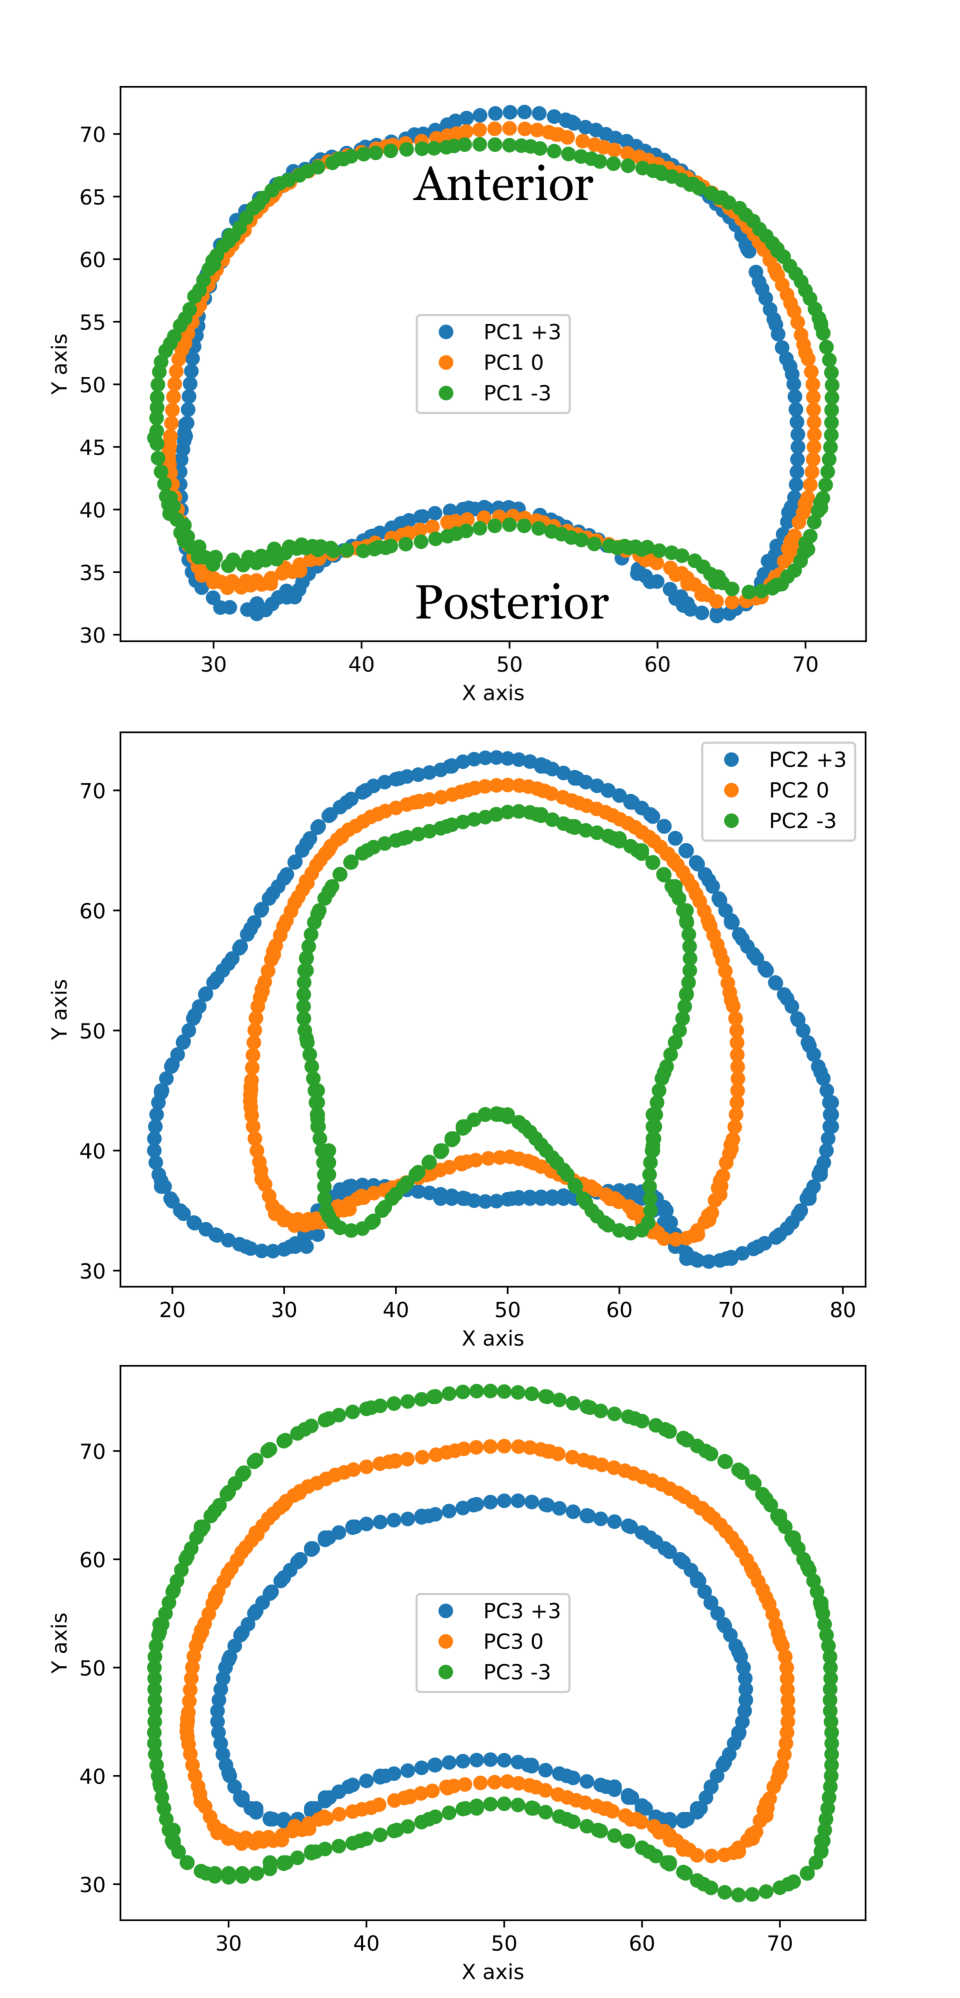
\includegraphics[width=.65\textwidth]{Chapters/Chapter_PCA_images/PC1_2_3_AxialSlice.pdf}
  \caption{Axial views of the mid slice of the vertebral models from the first three principal components, showing the mean, +3 and -3 standard deviations away from the mean. Showing how the geometry is captured in the first three principal components.}
  \label{fig:PC1_2_3_AxialSlice}
\end{figure}

\begin{figure}[p]
  \centering
  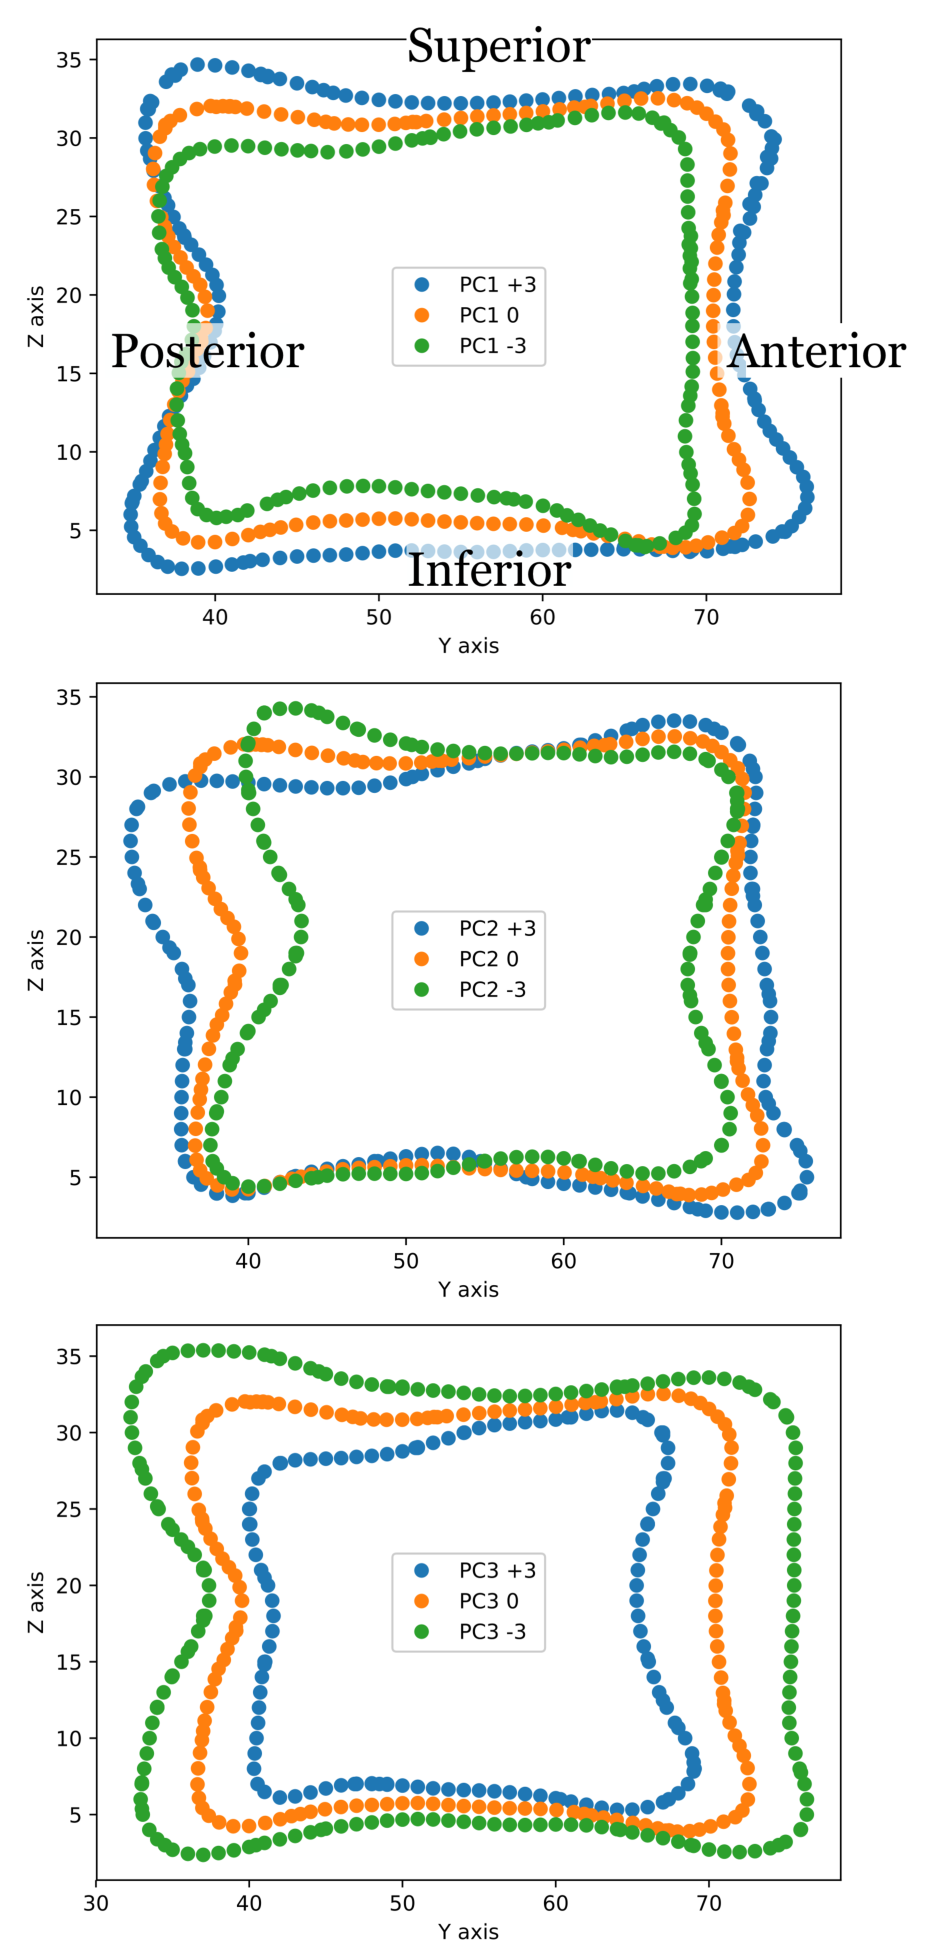
\includegraphics[width=.65\textwidth]{Chapters/Chapter_PCA_images/PC1_2_3_SagitalSlice.pdf}
  \caption{Sagittal views of the mid slice of the vertebral models from the first three principal components, showing the mean, +3 and -3 standard deviations away from the mean. Showing how the geometry is captured in the first three principal components.}
  \label{fig:PC1_2_3_SagitalSlice}
\end{figure}

\begin{figure}[p]
  \centering
  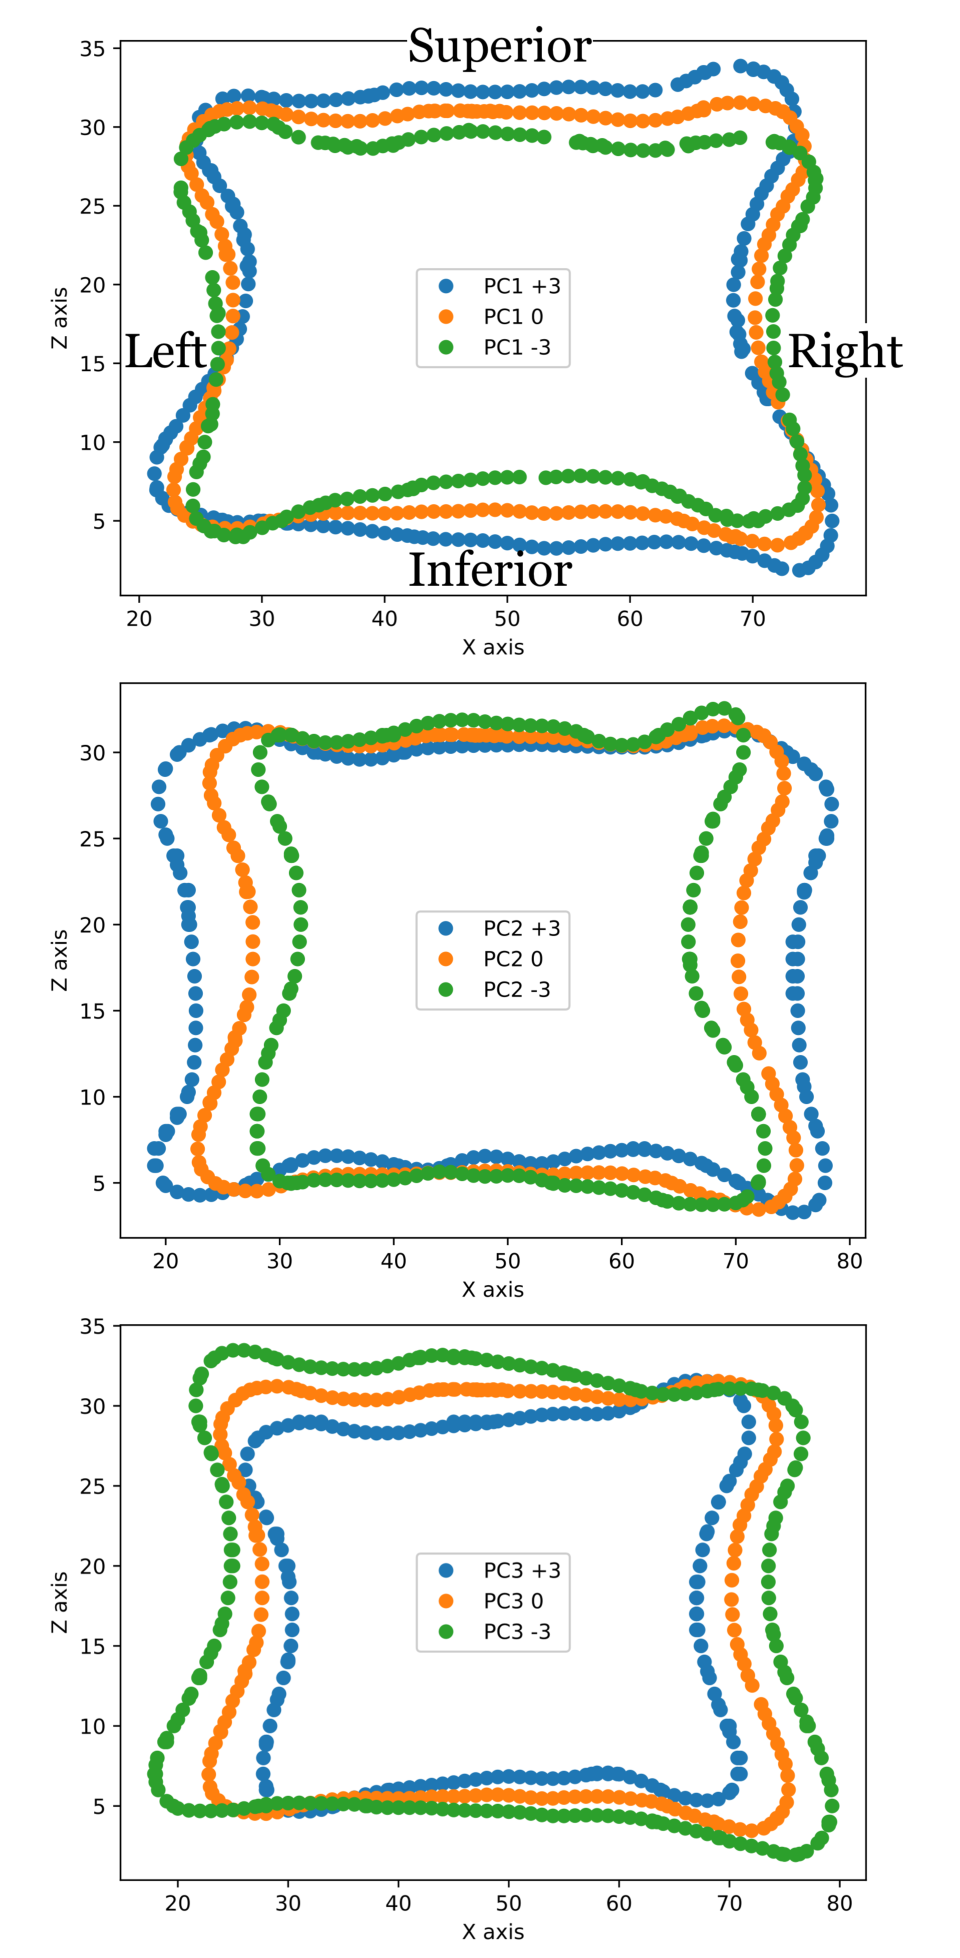
\includegraphics[width=.65\textwidth]{Chapters/Chapter_PCA_images/PC1_2_3_CoronalSlice.pdf}
  \caption{Coronal views of the mid slice of the vertebral models from the first three principal components, showing the mean, +3 and -3 standard deviations away from the mean. Showing how the geometry is captured in the first three principal components.}
  \label{fig:PC1_2_3_CoronalSlice}
\end{figure}



\begin{landscape}

\begin{table}[p]
  \centering
  \caption{The measurements of the 18 variables (abbreviations in \cref{tab:measurements}), shown as a fraction of the mean models measurements. Colouration shows the reduced measurements in red and larger measurements in green showing the geometric variation quantitatively.}
  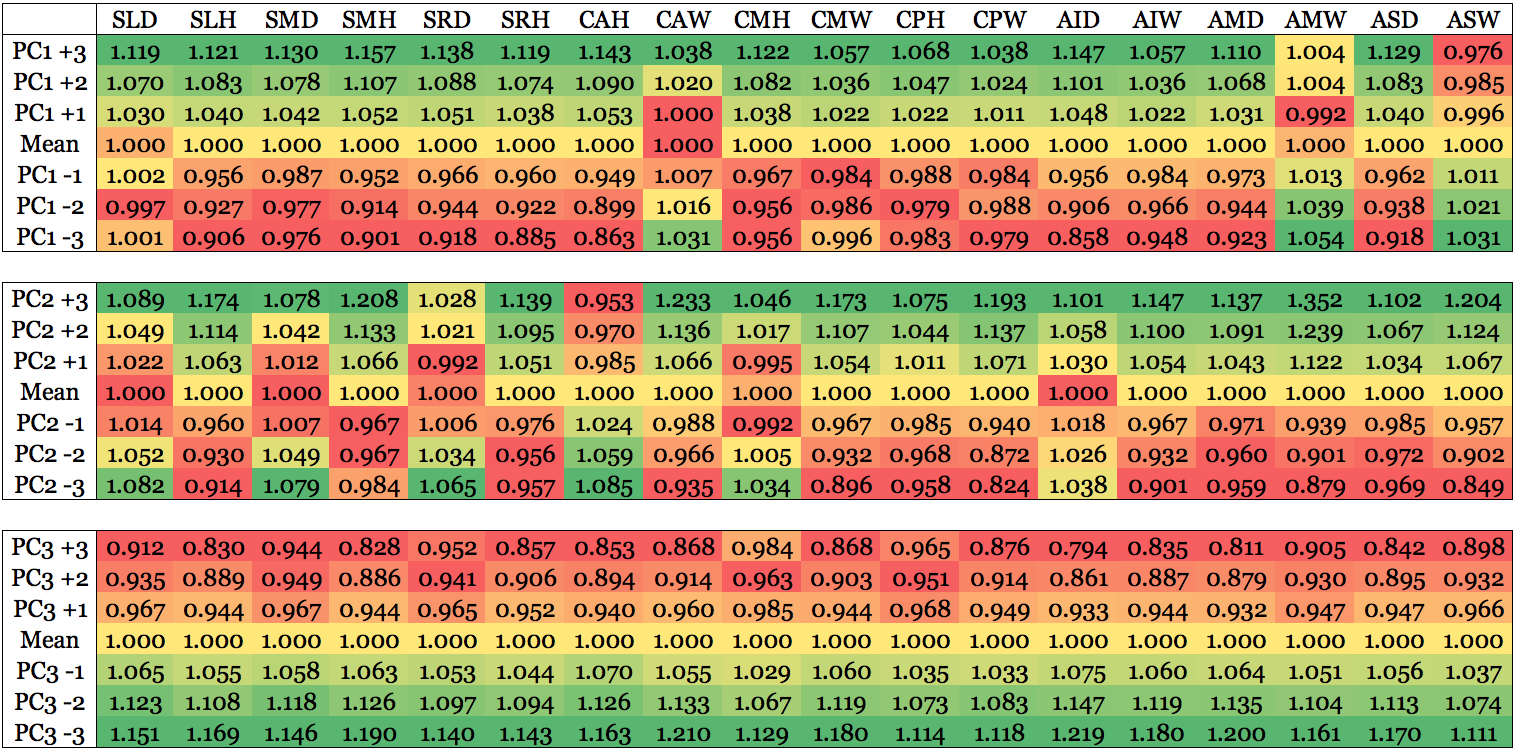
\includegraphics[width=1.7\textwidth]{Chapters/Chapter_PCA_images/pca_geo_table.png}
  \label{tab:pca_geo_tab}
\end{table}

\end{landscape}

General changes to the volume of the generated vertebral models can be seen in
\cref{fig:pca_vol}.  This shows a small and similar change to the volume of the
vertebrae in both PC1 and PC2, corresponding to general size changes and shape
changes repectively.  The majority of the volume changes are isolated to PC3,
which again captures size variation, with little change to the shape as seen
above.

\begin{figure}[h]
  \centering
  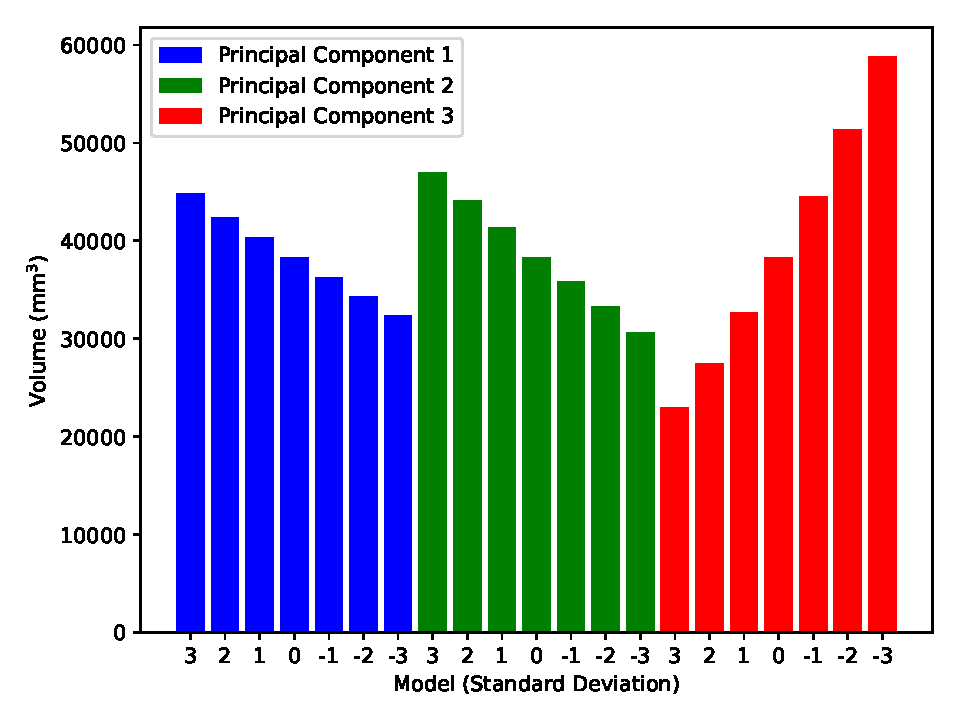
\includegraphics[width=.9\textwidth]{Chapters/Chapter_PCA_images/pca_vol.pdf}
  \caption{The vertebral body volume variation for the first three principal components, including the variation at $\pm$1, 2 \& 3 standard deviations away from the mean and including the mean.}
  \label{fig:pca_vol}
\end{figure}




\subsubsection{Greyscale \& Material Property Variation}

Variation in the greyscale background or material properties of the vertebrae
was the primary mode of variation, hence most greyscale variation being
captured in principal component 1.  Unlike the other modes of variation where
changes exist in the other two principal components, greyscale variation is
almost completely isolated to PC1, which can be seen in both the comparison of
the mean greyscale value for each model in \cref{fig:pca_gs} and the plots of
histograms in \cref{fig:pca1_histo,fig:pca2_histo,fig:pca3_histo}.  The range
of the mean greyscale values for PC1 are from the least dense at -3 SD away
from the mean with a mean greyscale value of 42, to a maximum of 162 at +3 SD
away from the mean.

However, despite the similarity in the mean of the greyscale variation for PC2
and PC3, the distribution varies significantly, seen in
\cref{fig:all_pc1_2_3_slice_gs_density}.  In PC2 and PC3 (although more clearly
noticeable in PC3) the density distribution shifts from the posterior to the
anterior of the vertebral body.  In PC2 this shift of dnesest material is from
anterior to posterior in the models from -3 SD to +3 SD, as the vertebrae
change in shape from L1-like to L5-like.  In PC3 the shift of the densest part
is form posterior to anterior with reducing vertebral body volume (from -3 to
+3 SD).  Meaning that the larger vertebrae have a much denser posterior portion
and less dense anterior, while the smaller vertebrae have a much denser
anterior portion with a less dense posterior/pedicle region The density
distribution in PC1's models in more uniform, with more general changes to the
density as described earlier, with the -3 SD vertebrae having the least dense
properties and +3 SD having the most dense.  At the more dense end of PC1 (+3)
the thickness of the cortical shell increases significantly compared to that of
the least dense (-3).  However, the contrast between the shell and the
cancellous regions remain similar, while the mean model's cortical shell is
less clearly defined.

\begin{figure}[h]
  \centering
  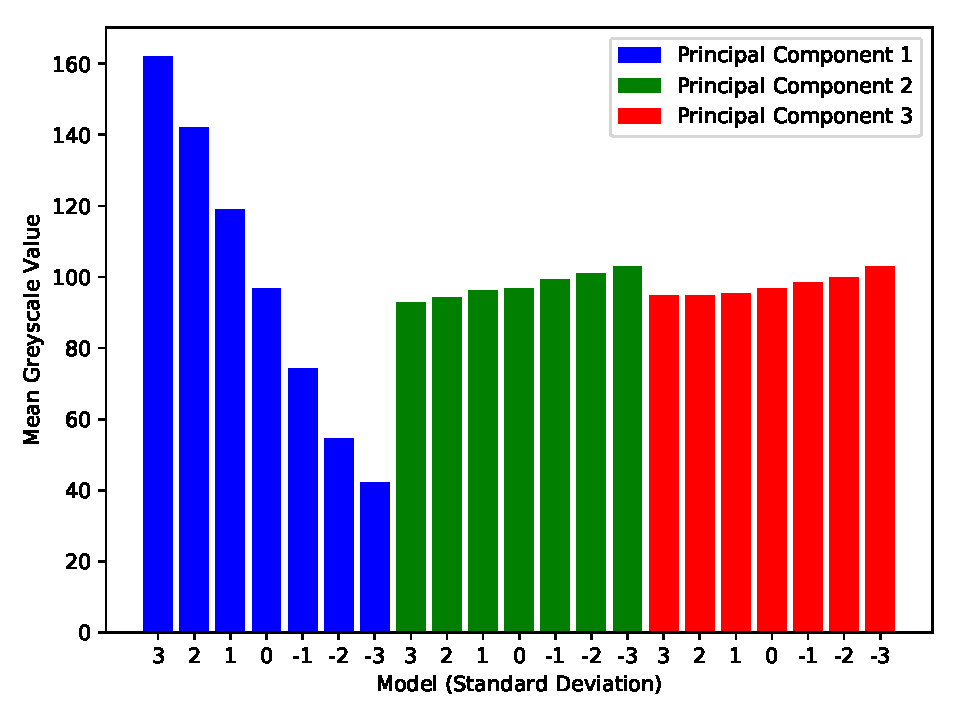
\includegraphics[width=.9\textwidth]{Chapters/Chapter_PCA_images/pca_gs.pdf}
  \caption{The mean greyscale variation for the first three principal
	components, including the variation at $\pm$1, 2 \& 3 standard
	deviations away from the mean and including the mean.}
  \label{fig:pca_gs}
\end{figure}

\begin{figure}[p]
  \centering
  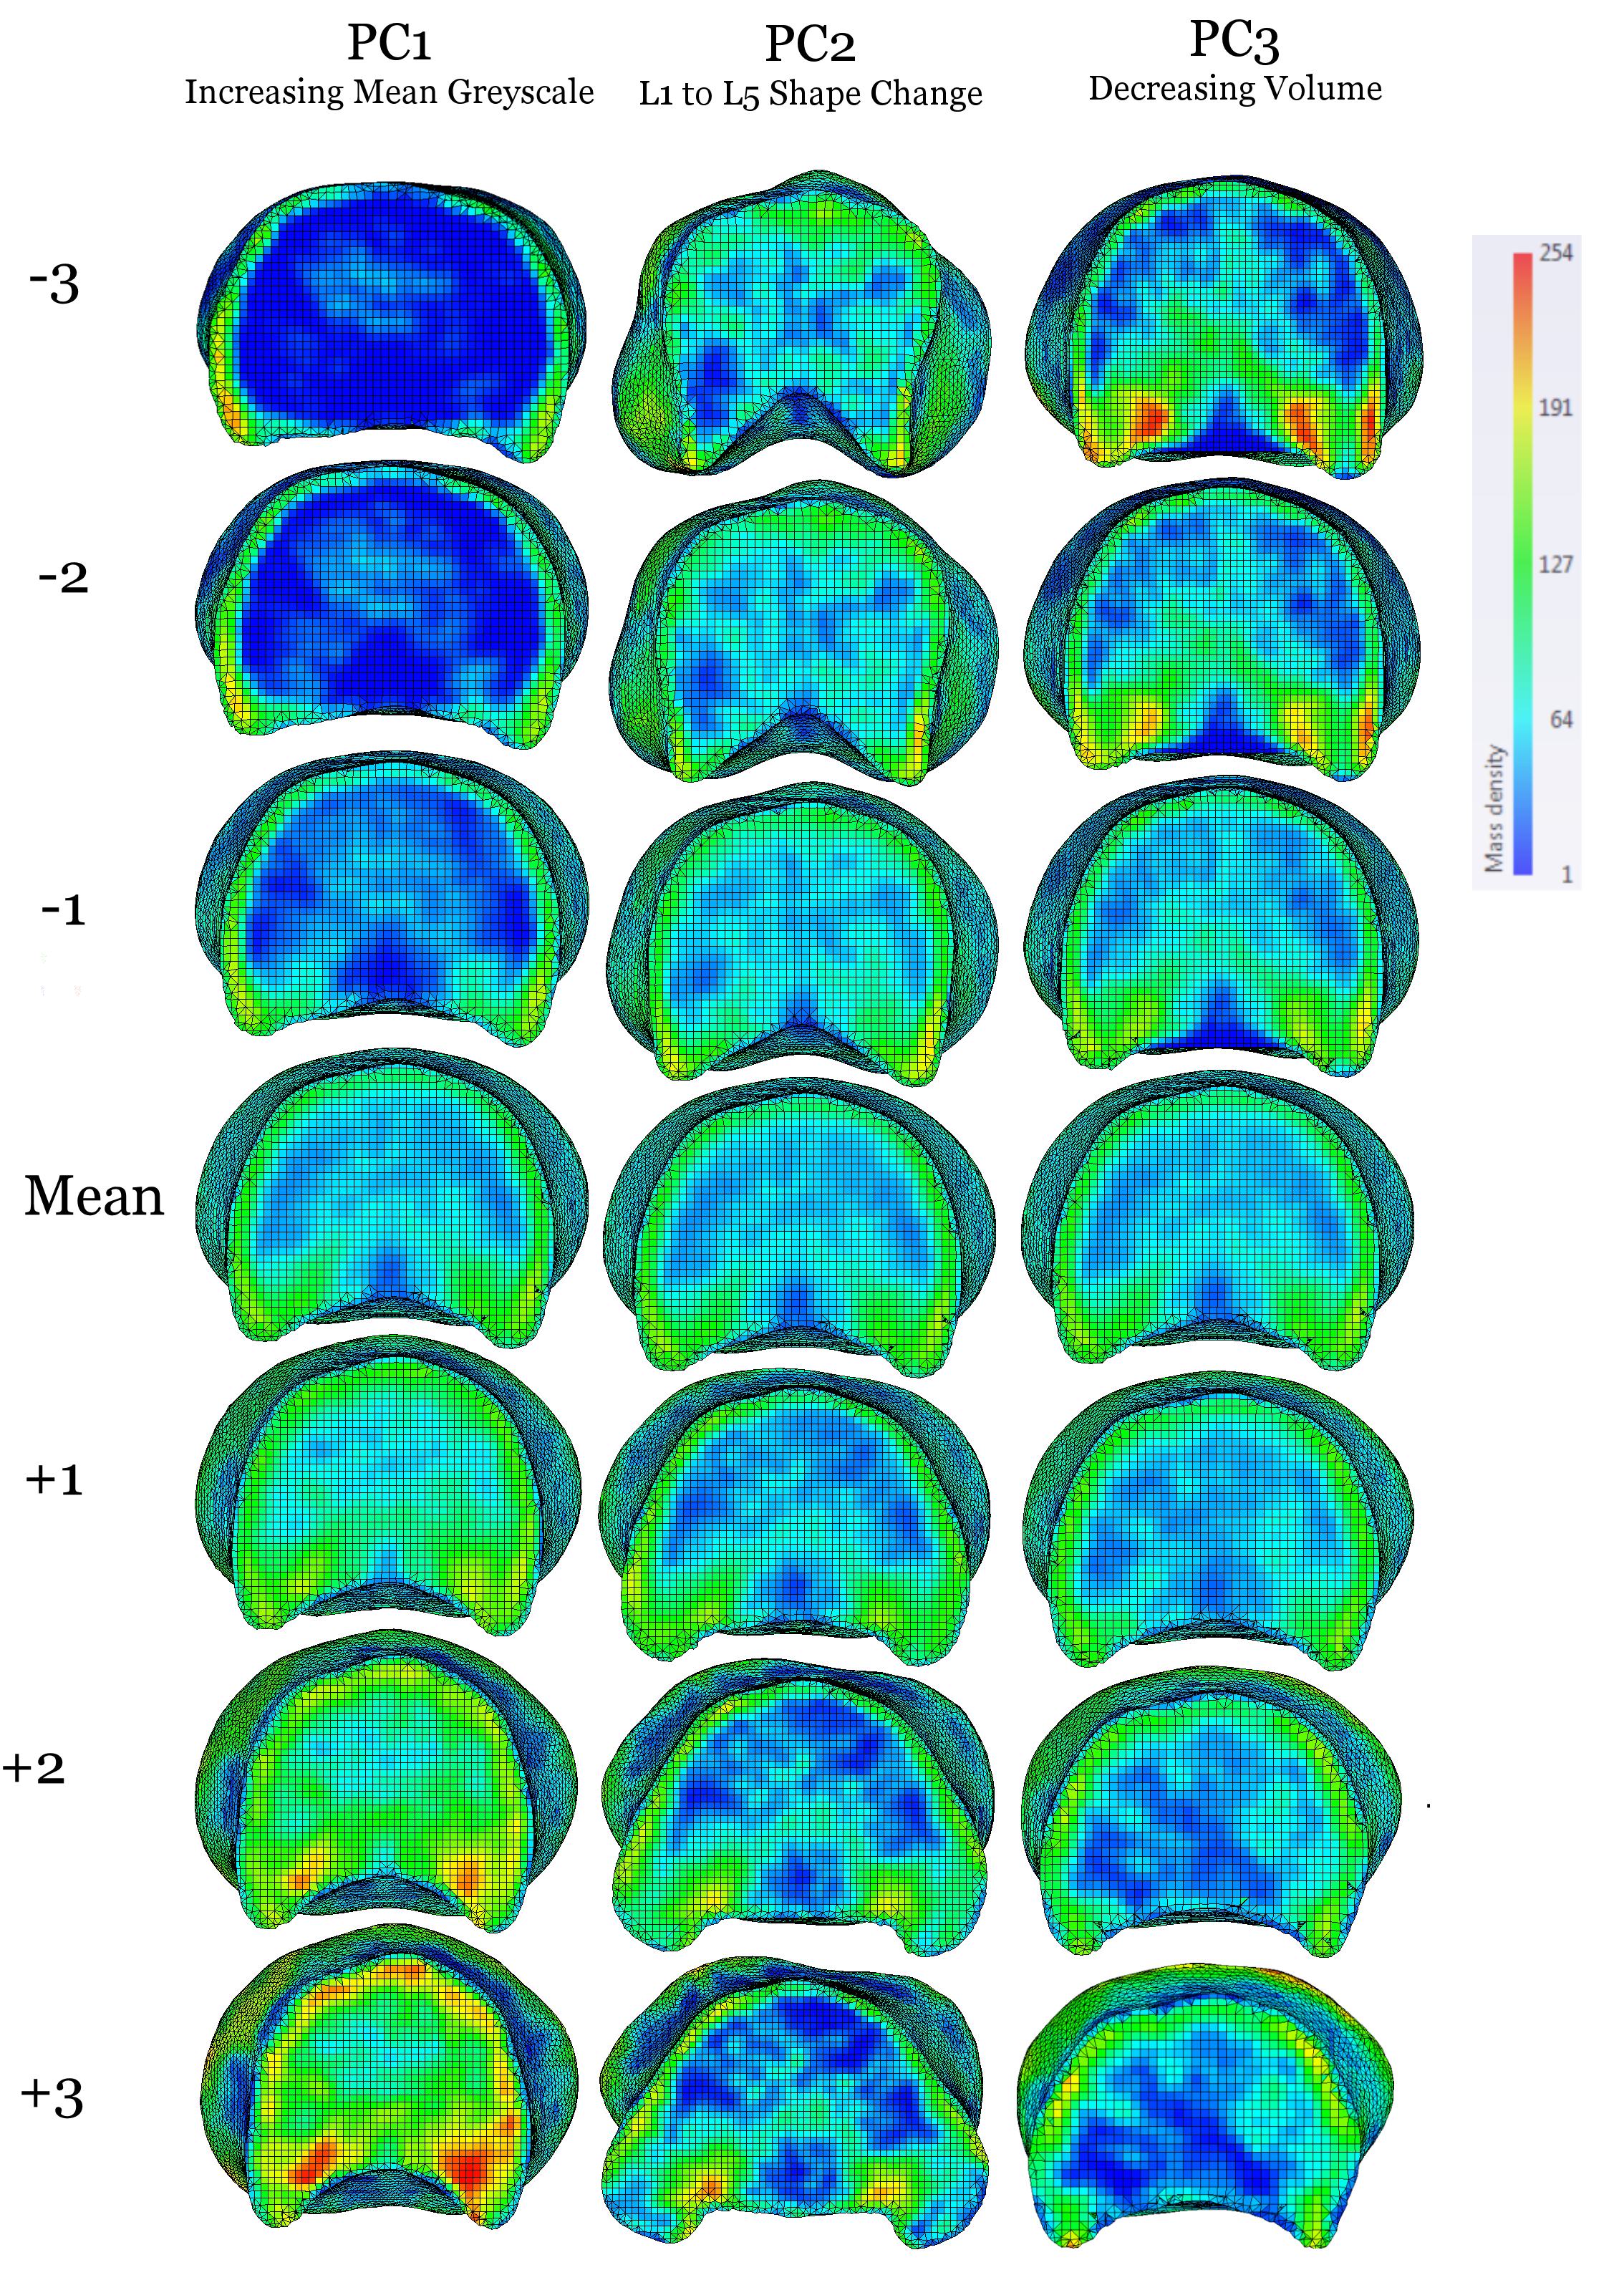
\includegraphics[width=.9\textwidth]{Chapters/Chapter_PCA_images/all_pc1_2_3_slice_gs_density.png}
	\caption[The variation in the greyscale distribution across the
	mid-slice of the vertebrae generated from the first three principal
	components.]{The variation in the greyscale distribution across the
	mid-slice of the vertebrae generated from PC1, PC2 and PC3, for each of
	the $\pm$1, 2 and 3 standard deviations from the mean.  Showing how the
	changing distribution of the greyscale, even for PC2 and PC3 where the
	mean greyscale variation is minimal.  Red colours indicate denser bone
	and blue colours indicate the least dense bone.}
  \label{fig:all_pc1_2_3_slice_gs_density}
\end{figure}

\subsubsection{Resulting Stiffness Variation}

The variation in the resulting stiffness of the generated model for principal
component 1 can be seen in \cref{fig:pca_stiff,tab:stiffness_gen_models}. The
trends within the different principal components  match closely with the
variation seen in the mean greyscale which can be seen in \cref{fig:pca_gs}.
This suggests a stronger relationship between the greyscale background and the
resulting stiffness of the models than any of the other variations in the
generated models when loaded centrally and without augmentation.

\begin{figure}[h]
  \centering
  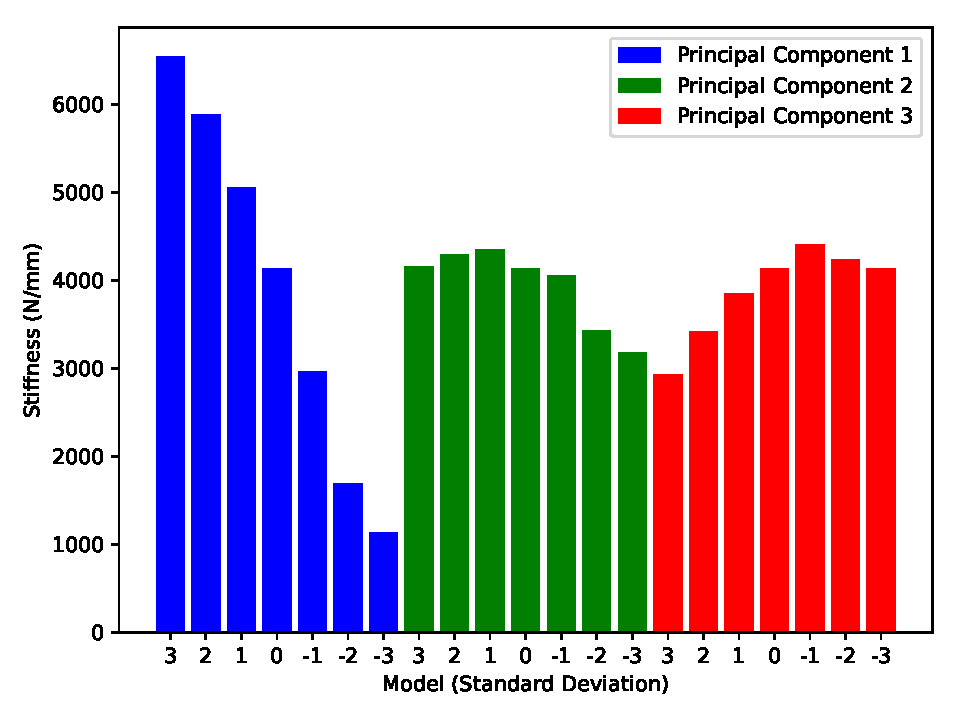
\includegraphics[width=.9\textwidth]{Chapters/Chapter_PCA_images/pca_stiff.pdf}
  \caption{The stiffness variation for the first three principal components,
	including the variation at $\pm$1, 2 \& 3 standard deviations away from
	the mean and including the mean.}
  \label{fig:pca_stiff}
\end{figure}

\begin{table}[h]
\centering
\caption{The stiffness of the generated models from PC1, 2 and 3, showing the fractional change to the mean model in each case.}
\label{tab:stiffness_gen_models}
\begin{tabular}{c|c|c}
Model  & Stiffness (N/mm) & Fractional Change from the Mean \\ \hline \hline
PC1 +3 & 6543.38          & 1.582                           \\
PC1 +2 & 5887.75          & 1.424                           \\
PC1 +1 & 5059.89          & 1.224                           \\
Mean   & 4134.88          & 1.000                           \\
PC1 -1 & 2962.82          & 0.717                           \\
PC1 -2 & 1696.47          & 0.410                           \\
PC1 -3 & 1131.86          & 0.274                           \\ \hline
PC2 +3 & 4159.29          & 0.980                           \\
PC2 +2 & 4291.53          & 0.831                           \\
PC2 +1 & 4355.98          & 0.770                           \\
Mean   & 4134.88          & 1.000                           \\
PC2 -1 & 4051.57          & 1.006                           \\
PC2 -2 & 3434.91          & 1.038                           \\
PC2 -3 & 3182.81          & 1.053                           \\ \hline
PC3 +3 & 2930.69          & 0.709                           \\
PC3 +2 & 3420.55          & 0.827                           \\
PC3 +1 & 3846.57          & 0.930                           \\
Mean   & 4134.88          & 1.000                           \\
PC3 -1 & 4409.05          & 1.066                           \\
PC3 -2 & 4240.58          & 1.026                           \\ \hline
PC3 -3 & 4141.31          & 1.002                          
\end{tabular}
\end{table}

\subsection{Augmentation in Generated Models}


The general effect of augmentation in the generated vertebrae can be seen in
\cref{fig:pca_percent_fill_pc1,fig:pca_percent_fill_pc2,fig:pca_percent_fill_pc3},
with the effect on stiffness variation isolated to the variation seen in each
principal component.  The vertebrae described by PC1 show an increase in
stiffness with increasing cement fill volume, except for the negative standard
deviations away from the mean, where a reduction in stiffness is seen for all
cement fill volumes.  A bimodal relationship is also seen in the vertebrae
generated from PC2 when augmentation is simulated.  Here, positive standard
deviations from the mean show a more pronounced increase in the stiffness at
the larger fill volumes when compared to the negative standard deviations.  The
bimodal distribution continues in PC3 where the increasingly negative standard
deviations have a more noticeable increase in the stiffness at higher cement
fill volumes, correlating with the vertebrae with larger vertebral body
volumes.

\begin{figure}[h]
  \centering
  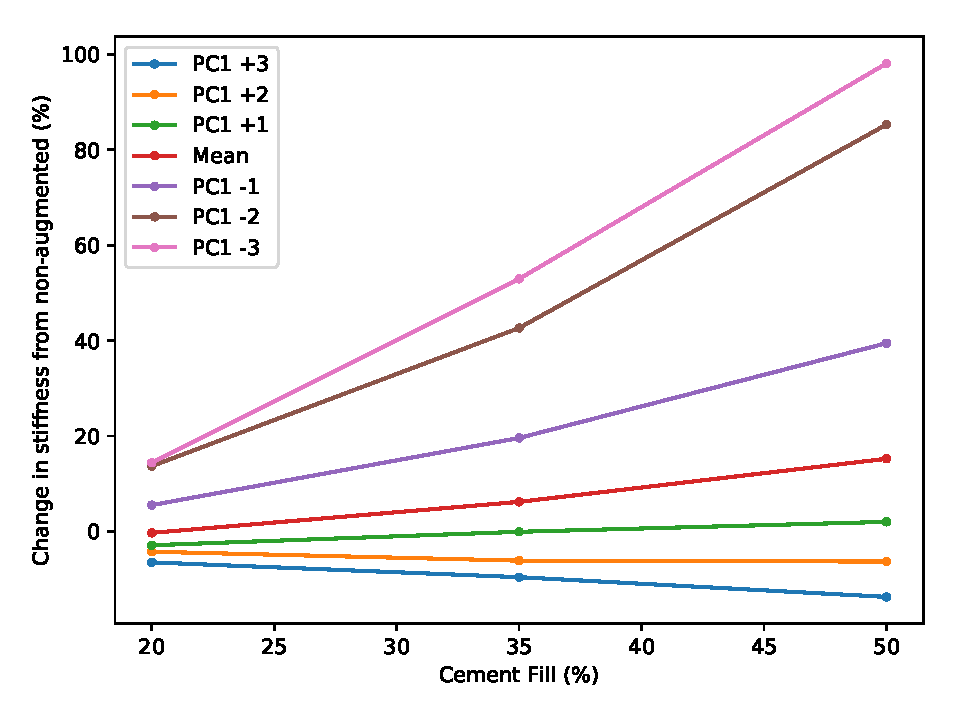
\includegraphics[width=.9\textwidth]{Chapters/Chapter_PCA_images/pca_percent_fill_pc1.pdf}
  \caption[Effect of augmentation in principal component 1.]{The effect of
	augmentation on vertebral stiffness in the vertebrae generated
	vertebrae from principal component 1, for 20, 35 and 50 percent fill
	volume. Shows the change from the non-augmented stiffness increasing
	with fill volume, with a more pronounced effect seen in the less dense
	vertebrae (-1, -2 \& -3 S.D. from the mean).}
  \label{fig:pca_percent_fill_pc1}
\end{figure}

\begin{figure}[h]
  \centering
  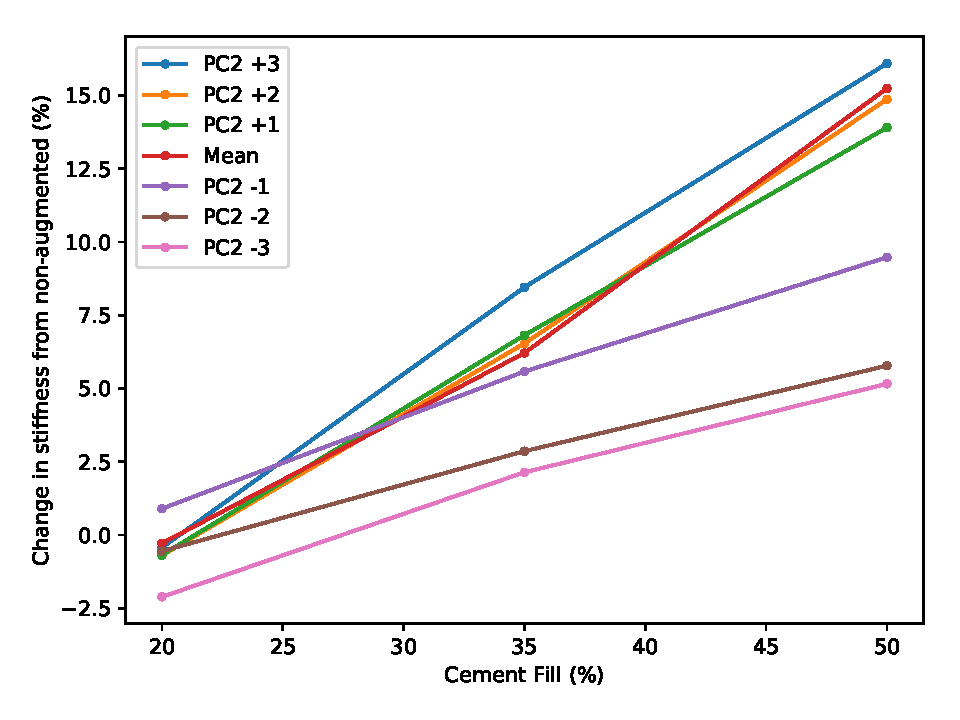
\includegraphics[width=.9\textwidth]{Chapters/Chapter_PCA_images/pca_percent_fill_pc2.pdf}
  \caption[Effect of augmentation in principal component 2.]{The effect of
	augmentation on vertebral stiffness in the vertebrae generated
	vertebrae from principal component 2, for 20, 35 and 50 percent fill
	volume. Shows the change from the non-augmented stiffness increasing
	with fill volume, with a more pronounced effect seen in the positive
	standard deviations away from the mean.}
	\label{fig:pca_percent_fill_pc2}
\end{figure}

\begin{figure}[h]
  \centering
  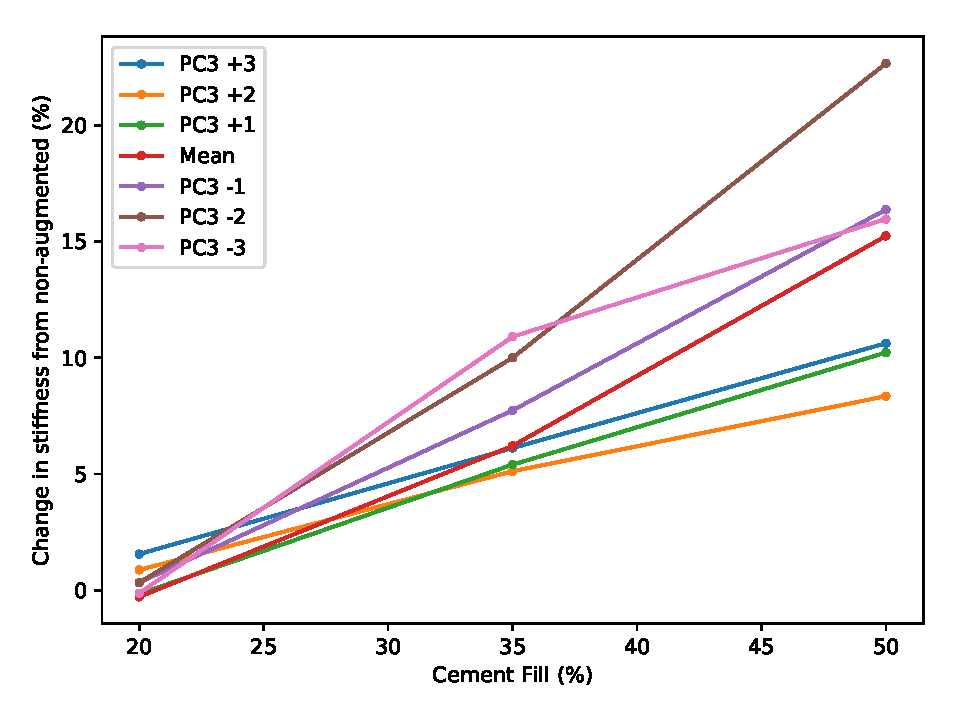
\includegraphics[width=.9\textwidth]{Chapters/Chapter_PCA_images/pca_percent_fill_pc3.pdf}
  \caption[Effect of augmentation in principal component 3.]{The effect of
	augmentation on vertebral stiffness in the vertebrae generated
	vertebrae from principal component 3, for 20, 35 and 50 percent fill
	volume. Shows the change from the non-augmented stiffness increasing
	with fill volume, with a more pronounced effect seen in the negative
	standard deviations away from the mean (larger volume).}
  \label{fig:pca_percent_fill_pc3}
\end{figure}


\subsubsection{Loading Position Effect on Augmentation }


The effect of loading position on the generated vertebral stiffness for
non-augmented vertebrae is similar to the effect seen with human vertebral
models seen in \cref{Chapter_HT} and is shown in \cref{fig:AP_LP_non_aug},
looking at posterior to anterior loads.  Broadly, the stiffness is greatest
when the vertebral models are loaded centrally, reducing as loads are applied
at greater distances from the centre.

Posterior to anterior loads in PC1 show large reductions furthest from centre
loading points, with the effect greatest for the densest vertebrae (+3 S.D.)
and least for the least dense vertebrae (-3 S.D.).  This reduction in stiffness
at 20 mm away from the centre, posteriorly or anteriorly is proportional to the
stiffness when loaded centrally, with reductions of approximately 70 \% for all
standard deviations from the mean.

Principle component two shows a very similar response to loading for all of the
standard deviations away from the mean.

Finally, principal component three is mostly uniform, except at the posterior
loading points, where the negative standard deviation models (larger vertebral
body size) have a reduced effect of posterior loading.


The effect of loading position on the augmented vertebrae can be seen in
\cref{fig:AP_change_from_non_aug}, identifying the effect of posterior and
anterior loads, comparing the percentage change in stiffness from the
non-augmented models.  At 20 percent fill volume, loading position has little
effect on the response to augmentation, with the percentage change less than 5
\% for all but PC1, where only the -3 S.D. model shows a change compared to the
central loading position, with an increase in stiffness when loading
posteriorly.

At 35 \% fill trends become apparent which continue and become more noticeable
at 50 \% fill.  PC1 has a simple relationship where augmentation has a smaller
effect when loaded at the most posterior or anterior loading positions compared
to the centre for the negative standard deviations.  However, in the positive
standard deviations (the more dense vertebrae), the change in stiffness is
greater when loaded anteriorly compared to posteriorly and similar compared to
centrally loaded.

PC2 has a near uniform reduction in stiffness when loading posteriorly compared
to the central loading position when filled with 35 and 50 \% fill.  When
loaded anteriorly, augmentation has little effect on the negative standard
deviation models, where the response to augmentation is similar for each
loading point.  For the positive standard deviation models however, there is a
large increase in the anterior stiffness following augmentation, with a
doubling of the change in stiffness seen in the +3 S.D. model when loaded
anteriorly compared to centrally.

PC3 has a similar response to augmentation at different loading points to PC2,
where posterior loads have little effect, or a reduced response compared to
central loading, except for the +3 S.D. model, where augmentation has the
greatest effect on stiffness when loaded posteriorly.  Augmentation increased
the stiffness most when loaded anteriorly for the negative standard deviations,
representing the largest vertebral body volumes.

\begin{figure}[p]
  \centering
  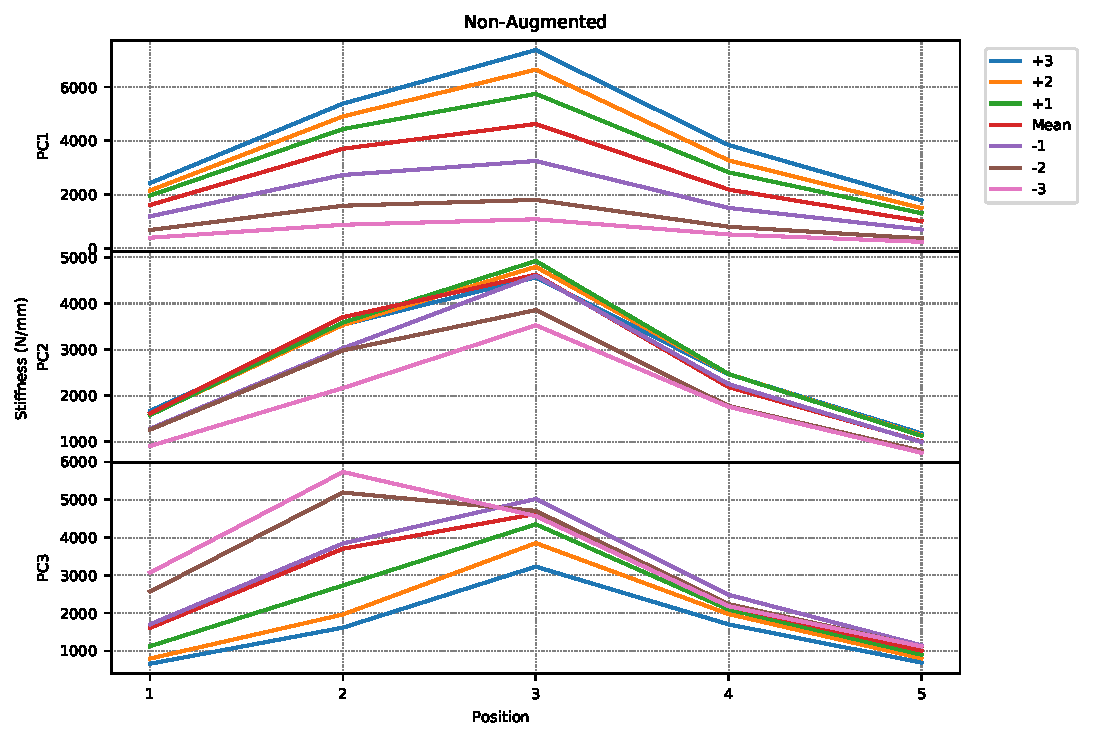
\includegraphics[width=.9\textheight, angle=90]{Chapters/Chapter_PCA_images/AP_LP_non_aug.pdf}
  \caption[Effect of loading position on the vertebral stiffness.]{Effect of
	loading position on the vertebral stiffness for PC1, PC2 and PC3 from
	posterior to anterior loading points. Loading point 1 and 2 are 20 mm
	and 10 mm posterior of the central loading point respectively, loading
	point 3 is the central position and load points 4 and 5 are 10 mm and
	20 mm anterior, respectively. }
  \label{fig:AP_LP_non_aug}
\end{figure}

\begin{figure}[p]
  \centering
  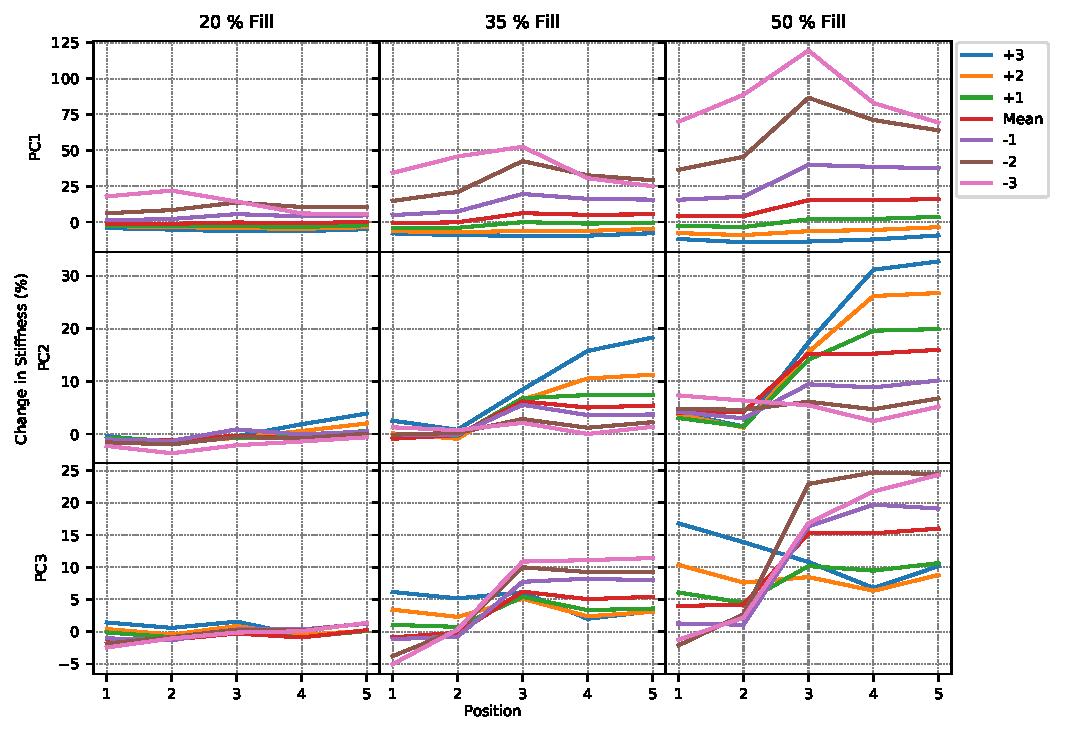
\includegraphics[width=.9\textheight, angle=90]{Chapters/Chapter_PCA_images/AP_change_from_non_aug.pdf}
  \caption[Effect of loading position on the augmented vertebral
	stiffness.]{Effect of loading position on the augmented vertebral
	stiffness for PC1, PC2 and PC3, and 20, 35 and 50 \% fill from
	posterior to anterior loading points. Loading point 1 and 2 are 20 mm
	and 10 mm posterior of the central loading point respectively, loading
	point 3 is the central position and load points 4 and 5 are 10 mm and
	20 mm anterior, respectively. }
  \label{fig:AP_change_from_non_aug}
\end{figure}
	
\subsubsection{Effect of Injected Cement Volume, Shape \& Position}		


\pagebreak


\section{Discussion} \label{pca_disc}

\subsection{Validation}

The models generated using the statistical shape modelling approach represent
the input set well with the range of measurements taken matching closely to the
range of measurements taken from the input set. The 18 measures of the geometry
describe the geometry well, with the most important measurements being ones
describing wedge shapes (with wedge fractures being the subject of many
vertebroplasty procedures) and the general shape changes between L1-like and
L5-like vertebrae. The range of variation within 1 standard deviation (all
possible combinations of the PC1, 2 and 3) captures most of the variation seen
in the input set, with an expectation that the remaining variation not captured
in 1 SD would be captured in the other two standard deviations. In a few cases
models produced variation that was not seen in the experimental input set; a
possibility here is that the combinations of principal components used to make
that model were unnatural, with another possibility being that with a larger
and therefore more varied input set such variation would be seen. However, the
models used in the remaining investigations were from principal components in
isolation, which all fell within the range of the input set. Finally, in
addition to the range being well represented, the measurements of the mean
generated model align closely with the mean of the input set measurements,
suggesting that the models are not skewed to one end of the variation
spectrum



in between ones

\subsection{Variation}

\subsection{Response to Augmentation}

The response to small quantities of cement injected into the vertebrae is
small. This is shown when comparing 20 \% fill volumes to 35 and 50 \% fill,
where an increase in the stiffness is barely seen and only in the least dense
vertebrae.  Attempts to understand the effect that the position of small
volumes of cement (12 \% fill) has on the stiffness of the vertebrae shows
sensible effects although a small percentage change to the stiffness of the
vertebra compared to central positions of the cement volume.



Moving the cement volume in a lateral, left to right direction showed a
reduction in stiffness when at the extremes of the vertebra, where the yielding
interface of the cement volume encroached on the denser cortical shell defined
by the greyscale background of the model.  The effect of the intermediate
cement positions had a near symmetrical appearance - to be expected from the
near symmetrical mean vertebra from the input set.

Inferior to superior movements of the cement showed a small change to the
stiffness with a 2 \% increase to the superior of the vertebra, though a
reduction when at the topmost point of the vertebra.  This can be explained by
understanding the greyscale distribution of the model background or the
material properties of the elements.  The element found in the centre of the
vertebra are less dense and have a lower Young's modulus; when the cement was
positioned in the centre and near superior, less of the low Young's modulus
elements were exposed, resulting in an increased stiffness.

Moving the cement volume in a posterior to anterior direction showed a
reduction in stiffness when at the extremes of the vertebra similarly to the
lateral movements.  Away from the extremes, the stiffness rose to the anterior
of the vertebra, where the bone is less dense in both natural specimens and
these PCA generated models.  While this would suggest that vertebroplasty
injections should always aim to the anterior of the vertebra (for purely
stiffness increasing reasons, not just safety), the percentage change in
stiffness from the least stiff - most posterior to the stiffest position is a
mere 3 \%.  Given that the most stiff position still had a reduction of 13 \%
compared to the non-augmented vertebrae, it suggests other factors may be more
important and that the cement position, at least for small quantities of cement
have little effect.

Compounding these results with the effect of cement position when varying the
loading position... %TODO finish sentance

The effect of increasing the volume of the internal cement volume of the first
three principal components affected the different models differently depending
on what type of variation was found within that principal component.  As
described previously small volumes of cement had little effect on the stiffness
behaviour of the vertebral models, this extended to the 20 \% models where
little to no increase in the stiffness was seen.  At 35 \% fill effects of the
augmentation were seen, somewhat mirroring what was seen experimentally, where
increases in the stiffness were only seen beyond approximately 35 \% fill.  The
effect of increasing the cement from 20 through to 50 \% for the mean generated
vertebra had the effect of increasing the stiffness near linearly %TODO CHECK
Larger increases in the stiffness were seen for the negative standard
deviations away from the mean for PC1, where the main characteristic or mode of
variation was the mean greyscale values and the negative standard deviations
represented the least dense vertebra.  As expected these least dense vertebrae
had a large increase in stiffness, increasing further with the increased
volumes of cement.  Conversely, with the positive standard deviations away from
the mean of PC1 which contained the densest vertebrae in the set, the
increasing volume of cement reduced the stiffness of the vertebrae.  Again,
this mirrored what was seen experimentally, where those specimens that had the
highest bone volume fraction %TODO add where spines had the smallest response
to augmentation, with most showing a reduction in stiffness.  Computationally
this reduction in stiffness is due to the replacement of dense material with
high Young's moduli, to material with yielding properties and low Young's
moduli (the interface region), despite the Young's modulus of the cement region
itself being much higher than that of bone.  Experimentally, this reduction in
stiffness could be due to the greater level of damage caused when inserting
needles into the denser bone and other reasons described in \cref{Chapter_HT}.
%TODO check I've done this and the ref is correct.

%TODO add papers - back up what i'm saying below.
Despite some studies suggesting that small quantities of cement (less that 20
\%) are enough to increase or restore the stiffness or properties of fractured
vertebrae to that of the intact or natural vertebrae, the results presented
here suggest otherwise.  Additionally, these studies lack any validation of
experimental 


\subsection{Load Position Effect}\label{sec:lpe}

The effect of load position was investigated for the human tissue, where the
possible error in choosing the loading point of the model was $\pm$~1~mm given
the resolution.  The effect of moving the loading position within the 2~mm
range gave changes to the stiffness of approximately 5 \% (a small contribution
to the total possible error).  Here, the changes to the loading points are
$\pm$~10~mm and $\pm$~20~mm, giving loading points at approximately the
posterior boundary, the midpoint between the posterior boundary and the central
loading position and similar points on the anterior side.  This gave a
reasonable understanding of the effect of anterior and posterior loading for
the generated models, both with and without augmentation and more importantly a
more detailed understanding of the effect of augmentation on different types of
vertebra.

The response to loading for the different non-augmented vertebrae in PC1
followed the expectations given the incremental change in the density
distribution.  In PC2 near identical response from nearly all generated models
is explained by their similar volumes and similar mean greyscale values.  The
-1, -2 and -3 SD models that do not fit the same trends show a reduced
posterior density and hence show a reduced stiffness when loaded posteriorly.
A similar effect is seen in the PC3 vertebrae where the increased posterior
stiffness compared to the other models and the central loading position of -2
and -3 SD models is explained through a large increase in the posterior
density.The increased anterior density for the +3 and +2 models in PC3 seem to
have little effect on anterior loading.

The response to loading position when the vertebrae have certain fill volumes
of cement show interesting results which are not obvious without loading at
different positions.  At 20 \% fill volume the response to different loading
position is small, changes and patterns that are present are merely amplified
through the addition of larger volumes of cement.  At 35 \% fill the effect of
the loading position is clear, and mimics (to a smaller degree) what is seen in
the 50 \% fill volume models.  The change in stiffness for PC1 at 50\% fill
with anterior and posterior loads shows a reduced increase in stiffness
compared to the central loading position in the negative (less dense) SD
models.  However, there was still a larger response to augmentation in the -2,
-1, mean and +1 SD models when loaded anteriorly compared to posteriorly,
suggesting that models with less dense anterior portions have increased
responses to augmentation when loaded anteriorly.  The most dense vertebral
models in PC1 (+3, +2 SD) show little response to augmentation in general, with
no clear effect of changing the loading position.

The increase in change in stiffness for the positive standard deviation models
in PC2 when loaded anteriorly may be a combination of the shape of the models
(the L1 to L5 shape shift from -3 to +3 SD) and the shifting density
distribution from anterior to posterior with -3 to +3 SD.  Given that the
anterior portion of the +1, +2 and +3 SD models within PC2 have a lower
anterior density, the support given to this region through augmentation may
explain the increased change in stiffness.  Additionally, the positive standard
deviations exhibit greater anterior height.  The combination of the additional
height and density may explain why the increase in stiffness reaches a maximum
of +33 \%, greater than the +25 \% maximum seen in anterior loading of the PC3
vertebrae that also show the shifting density distribution.  Posterior loads
have little effect to the vertebrae in PC2, with all generated models showing a
very similar response, potentially adding weight to the idea that the anterior
loading response is shape driven.  The negative standard deviation models in
PC2 show a near uniform response to the different loading position, this may be
due to the smaller size along with a smaller anterior height.  The reduced
height suggests an increase in density (given the near uniform mean greyscale
values for PC2), which, as with PC1 causes a reduced response to augmentation.

When loading is varied in PC3 there is a reverse relationship between the +2
and +3 vertebrae compared to the other models (+2 and +3 show a greater
response to posterior loads, others show greater response to anterior loads and
a reduced response to posterior loads). The main variable in PC3 is the size
variation, however given that the cement fill volume is a constant 50 \% the
cause of the varied response is likely the change in material properties. Like
PC2, this change in material properties is the shift in the density
distribution where smaller +2 and +3 vertebrae have a less dense posterior
region. This results in an increase in posterior stiffness following
augmentation for these models due the low stiffness/density of the posterior
region. The remaining vertebrae have very dense posterior regions, explaining
the reduction in posterior stiffness following augmentation - the same effect
seen in the densest vertebrae of PC1. Conversely, the reduced anterior density
explains the increase in stiffness following augmentation when loaded
anteriorly.


Further isolation of the variation in the principal components would aid the
understanding of the true cause of the different responses to augmentation, for
example the combination of shape and volume changes in PC2 and PC3 with the
density distribution changes. Potential risks of this however are that such
variation types do not exist in isolation, at least in this dataset, for
example a L1 to L5 shape variation may always exhibit the density shift.  This
may be due to the load sharing variation caused by the bending of the lumbar
region, where the central lumbar vertebra (L3) may experience more central
loading, with the L1 and L5 vertebrae experiencing anterior or posterior loads
depending on the degree of lordosis in the lumbar spine.  Another relationship,
that may be specific to this data set is the shift in the density distribution
with vertebral body volume.  This relationship extends from PC2 to PC3 where
the larger vertebra (likely L5 vertebrae) show an increased posterior density,
suggesting that that posterior experienced larger loads in the body.  Again,
like PC2, the smaller vertebrae in PC3 (likely L1 vertebrae) showed greater
anterior density and likely higher anterior loads in the body.
%TODO add refs to the PCA spine section papers
